
\documentclass[11pt]{article} 

\usepackage[utf8]{inputenc} 
\usepackage{geometry} 
\usepackage{graphicx}% http://ctan.org/pkg/graphicx
\usepackage{array}% http://ctan.org/pkg/array
\geometry{a4paper} 

\vspace{2cm}
\setlength{\parindent}{0cm}
\usepackage{graphicx,wrapfig,placeins}

\title{Disney BRDF}
\author{Chichi Francesco}

\begin{document}
\maketitle
\graphicspath{{img/}}
\section{Introduction}
	This project aims to implement the \textbf{Bidirectional Reflectance Distribution Function} developed by the Disney company. 

\newpage
\section{Bidirectional reflectance distribution function (BRDF)}
The bidirectional reflectance distribution function is a function $ f(x,i,o) $ that defines how light is reflected at an opaque surface (figure \ref{fig:reflect}), and is defined as the ratio of the differential reflected radiance over the
differential incident irradiance. 
In simple terms, the BRDF define the probability that a photon coming from a direction \textit{i} is reflected in a direction \textit{r}, after the collision with an opaque surface.
We can so define it as \cite{slide}:
$f(x,i,o)=\frac{\delta L_r(x,o)}{\delta E_i(x,i)} = \frac{\delta L_r(x,o)}{L_i(x,i)(n_x\cdot i) \delta \omega_i} $

\begin{figure} [ht]
	\centering
	
\includegraphics[width=0.5\linewidth]{img/reflect}
	\caption{A graphical example of the photon's reflection on an opaque surface.}
	\label{fig:reflect}
\end{figure}

A physically based specular BRDF is based on micro-facet theory, which describe a surface is composed of many micro-facets and each micro-facet will only reflect light in a single direction according to their normal(m) (figure \ref{fig:microfacet}) \cite{slide,microfacet} 

\begin{figure}[ht]
	\centering
	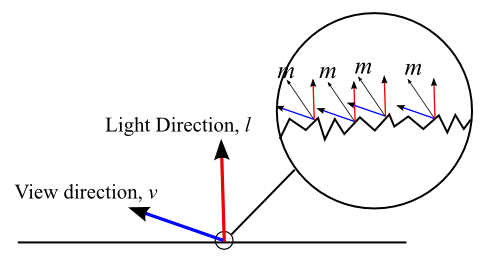
\includegraphics[width=0.5\linewidth]{img/microfacet}
	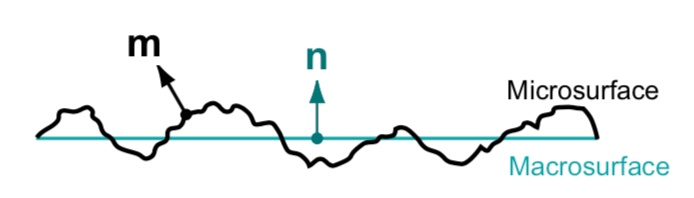
\includegraphics[width=0.5\linewidth]{img/microfacet2}
	\caption{A graphical example of the photon's reflection on the microfacets surfaces.}
	\label{fig:microfacet}
\end{figure}

So, the BRDF is essentially the "average" value of all these reflection events among all the micro-facets.
The microfacet reflection is then the normalized product of three terms:
$f_r(i,o)=\frac{F(i,h)D(h)G(h,i,o)}{4|n\cdot i||n\cdot o|}$\\
$h= \frac{i+o}{|i+o|}$ \\
Where F is the fresnel term, that take accounts for difference at grazing angle, the microfacet distribution D describes the statistical distribution of microfacets in a surface and the shadow-masking term G, that corrects for facets not visible from light or from the point of view (fig \ref{fig:visible})

\begin{figure}[ht]
	\centering
	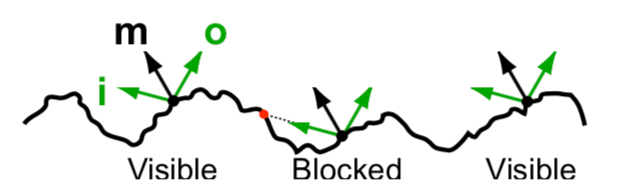
\includegraphics[width=0.5\linewidth]{img/visible}
	\caption{Example of the microfacet surface visibility.}
	\label{fig:visible}
\end{figure}


\section{Disney BRDF}
The Disney company studied and developed a custom BRDF, in order to increase the
richness of all of their materials while making lighting responses more consistent between materials and
environments and also wanted to improve artist productivity through the use of simplified controls.\\
In graphics, one of the most diffuse model for represent the Fresnel reflection $ (k_r) $ and transmission $ (k_t = 1 - k_r) $ is the Schlick's approximation:
$ k_r = k_s^0 + (1 - k_s^0)(1 - | n\cdot i|)^5$.
This term is used in the Lambert diffuse model $ diffuse + \frac{D(\theta_h)F(\theta_d)G(\theta_l,\theta_v)}{4cos\theta_lcos\theta_v} $, which give a good physical representation of the scene.
The problem, for the Disney company, was that this model is often too dark on the edges, and adding a Fresnel factor to make it more physically plausible only makes it darker.
The model developed aims to increase the refraction at gazing angles, the angle between the tangent to the surface and the outgoing ray, when the light enters and exits the sides of micro-facet surfaces.
The resultin diffuse model is the following:\\\\
$ \frac{baseColor}{\pi} (1 + (F_{D90} - 1)(1 - cos\theta_l)^5)(1 + (F_{D90} -1)(1 - cos\theta_v)^5)$\\\\
where  $F_{D90} = 0.5 + 2cos\theta_d^2$ \textit{roughness}\\\\
\subsection{Nomenclature}

\subsection{Diffuse model}

The resulting diffuse Fresnel have a redocted incident diffuse reflectance by 0.5 at gazing angles for smooth surfaces and an increased response by up to 2.5 for the rough ones.
\subsection{Specular D}
\subsection{Specular F}
\subsection{Specular G}
\subsection{yocto-gl Implementation}

\begin{table}[ht]
  \centering
  \begin{tabular}{ | c | c | c |}
    \hline
    path & const 0.6 gamma 2 & const 0.3 gamma 2 \\ \hline
    \begin{minipage}{.3\textwidth}
      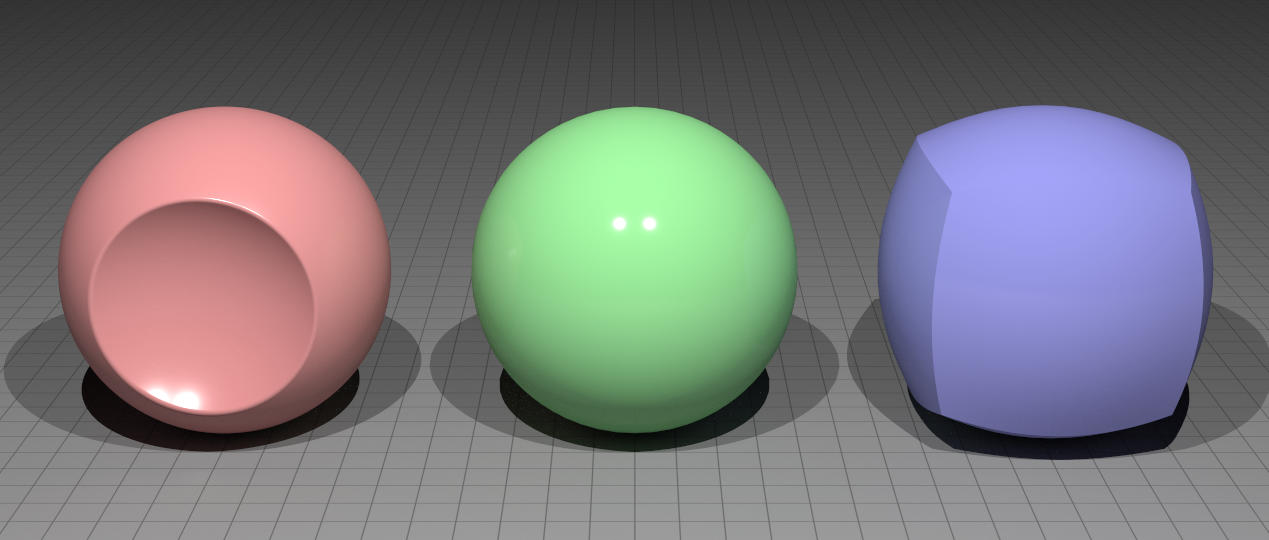
\includegraphics[scale=0.1]{img/obj/basic_pl/basic_pl.jpg}
    \end{minipage}
    &
    \begin{minipage}{.3\textwidth}
      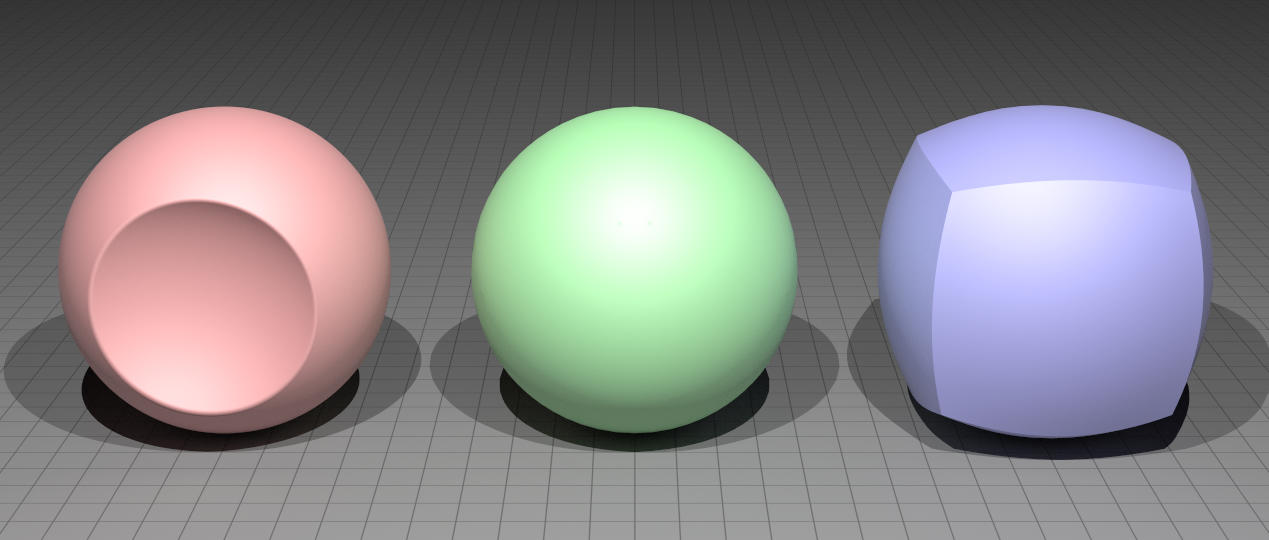
\includegraphics[scale=0.1]{img/obj/basic_pl/basic_pl_disney.jpg}
    \end{minipage}
    & 
    \begin{minipage}{.3\textwidth}
      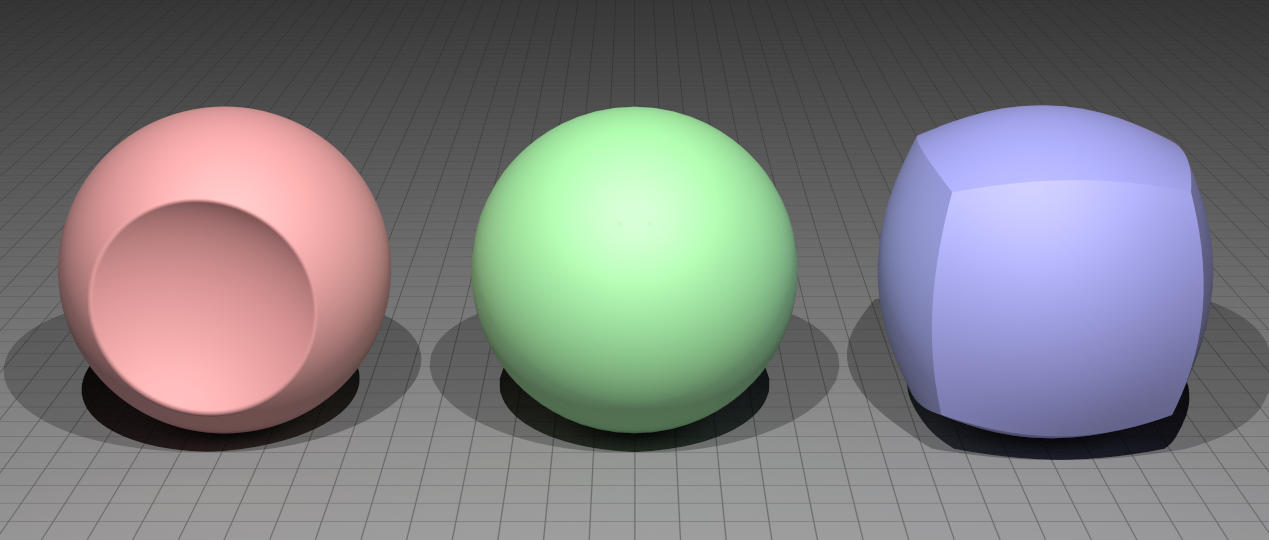
\includegraphics[scale=0.1]{img/obj/basic_pl/basic_pl_disney_dc03.jpg}
    \end{minipage}
    \\ \hline
  \end{tabular}
\end{table}
\begin{table}[ht]
  \centering
  \begin{tabular}{ | c | c | }
    \hline
    const 0.6 gamma 1 & const 0.3 gamma 1 \\ \hline
    \begin{minipage}{.3\textwidth}
      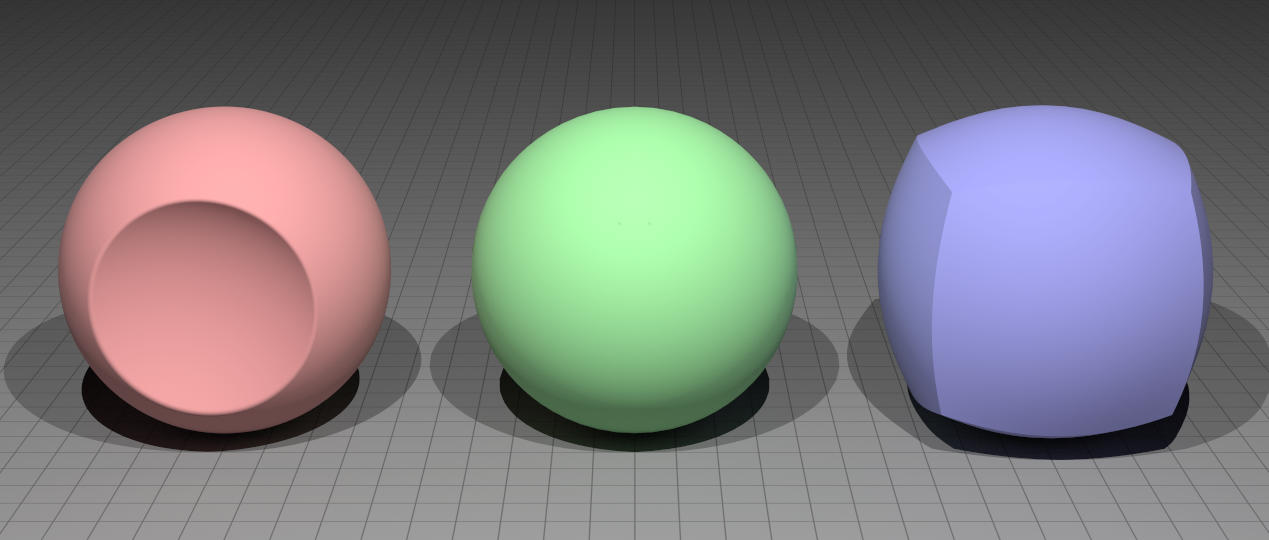
\includegraphics[scale=0.1]{img/obj/basic_pl/basic_pl_disney_dc03_dg1.jpg}
    \end{minipage}
    &
    \begin{minipage}{.3\textwidth}
      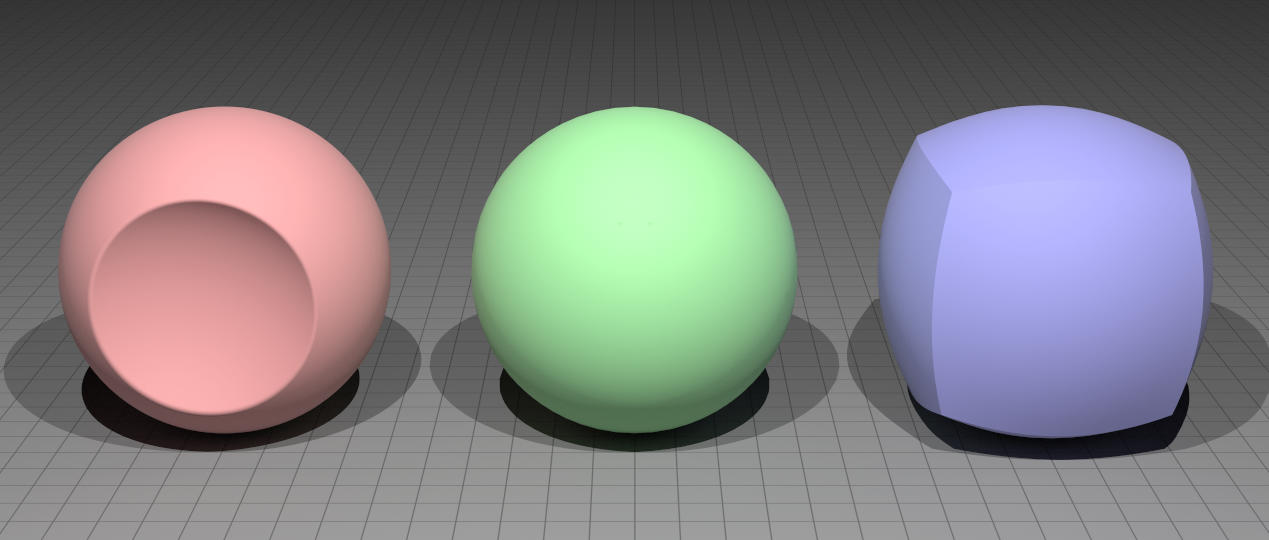
\includegraphics[scale=0.1]{img/obj/basic_pl/basic_pl_disney_dg1.jpg}
    \end{minipage}
    \\ \hline
  \end{tabular}
  \caption{\textit{basic\_pl} object rendered with the basic path tracer and with the one of Disney}\label{tbl:myLboro}
\end{table}



\section{Conclusions}
\section{Sperimental results}


\begin{table}[ht]
  \centering
  \begin{tabular}{ | c | c | c |}
    \hline
    path & const 0.6 gamma 2 & const 0.3 gamma 2 \\ \hline
    \begin{minipage}{.3\textwidth}
      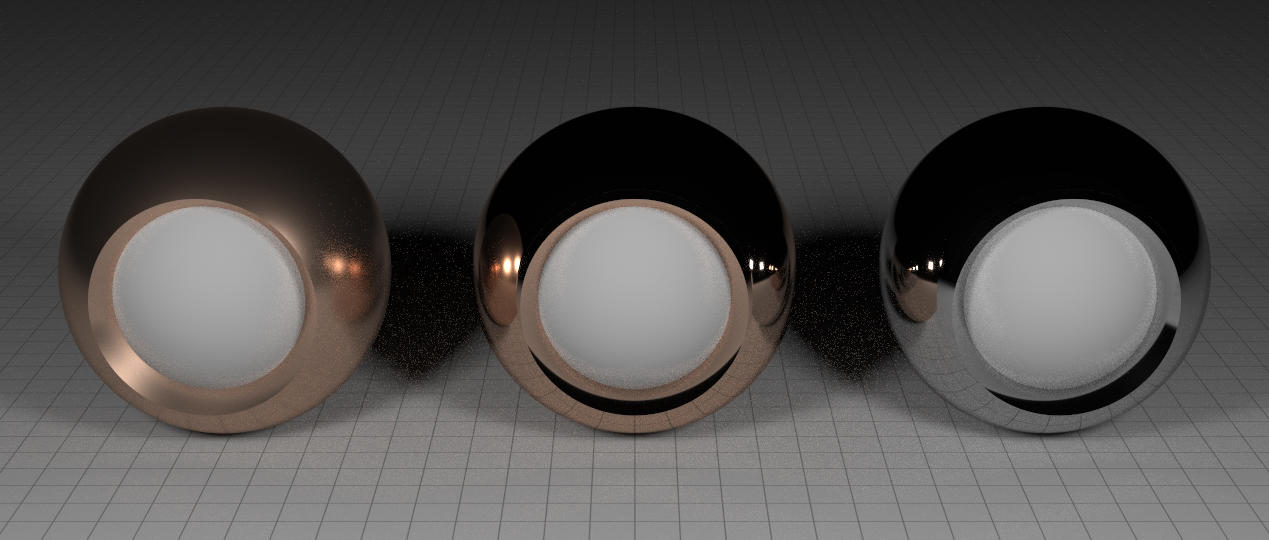
\includegraphics[scale=0.1]{img/obj/metals_al/metals_al.jpg}
    \end{minipage}
    &
    \begin{minipage}{.3\textwidth}
      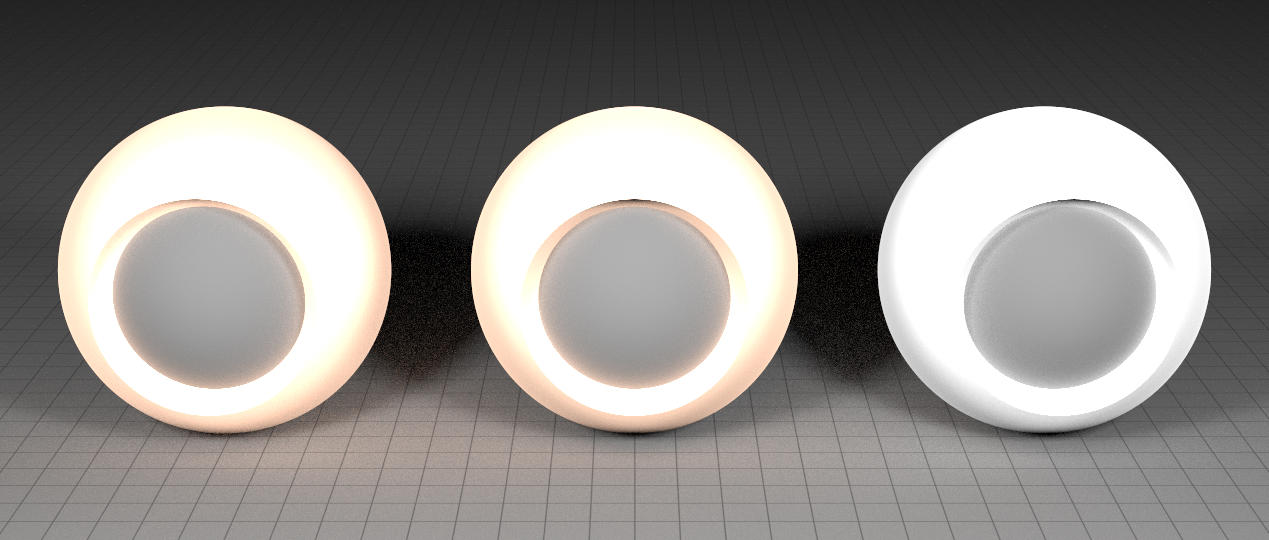
\includegraphics[scale=0.1]{img/obj/metals_al/metals_al_disney.jpg}
    \end{minipage}
    & 
    \begin{minipage}{.3\textwidth}
      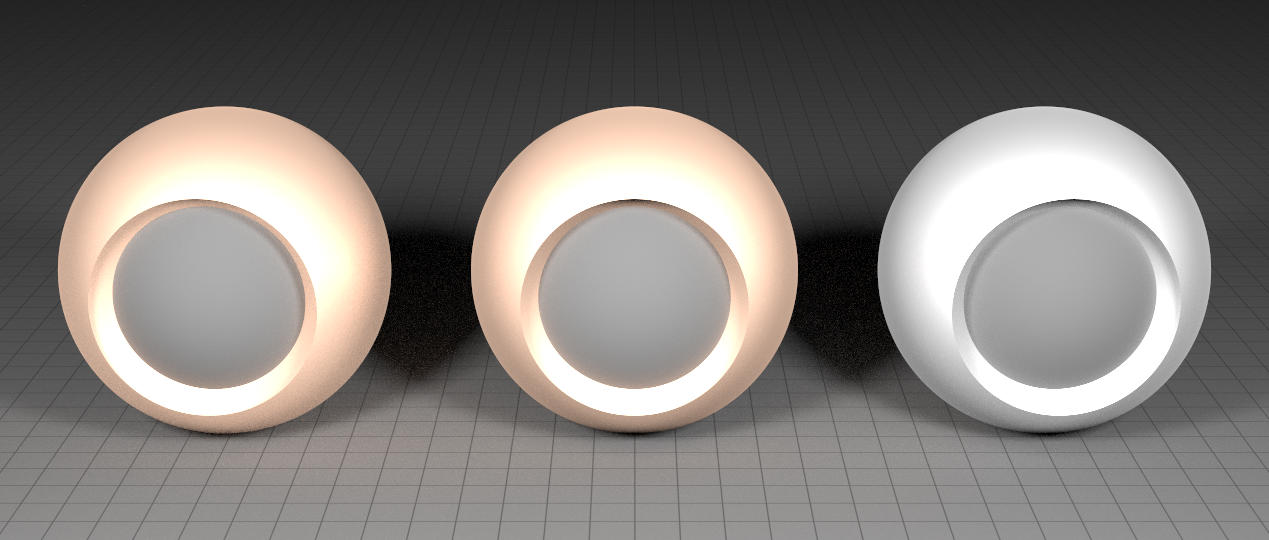
\includegraphics[scale=0.1]{img/obj/metals_al/metals_al_disney_dc03.jpg}
    \end{minipage}
    \\ \hline
  \end{tabular}
\end{table}
\begin{table}[ht]
  \centering
  \begin{tabular}{ | c | c | }
    \hline
    const 0.6 gamma 1 & const 0.3 gamma 1 \\ \hline
    \begin{minipage}{.3\textwidth}
      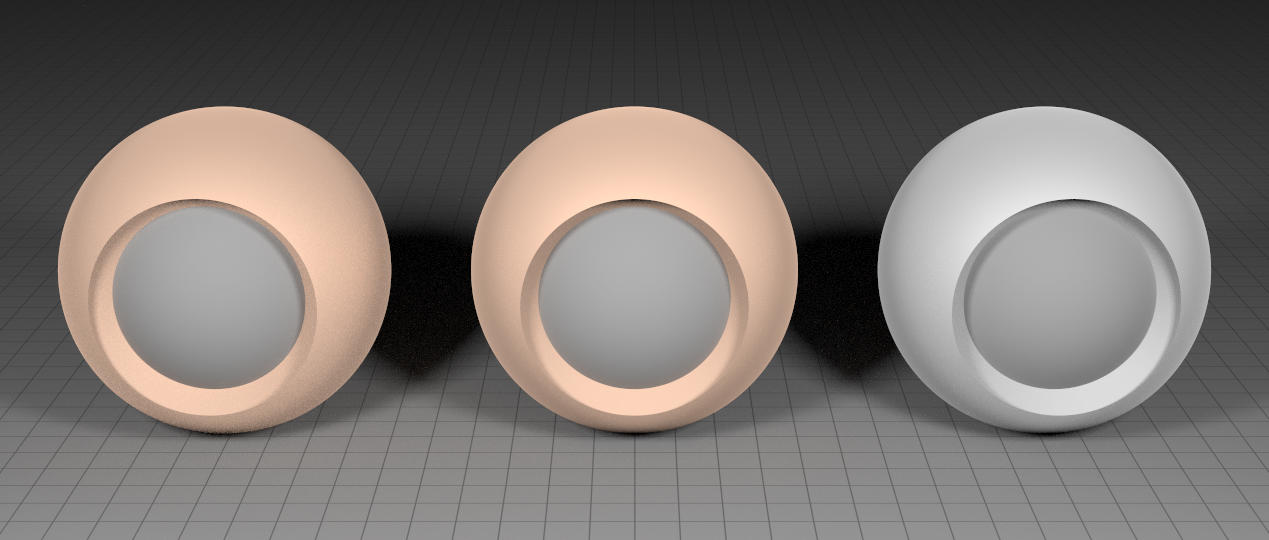
\includegraphics[scale=0.1]{img/obj/metals_al/metals_al_disney_dc03_dg1.jpg}
    \end{minipage}
    &
    \begin{minipage}{.3\textwidth}
      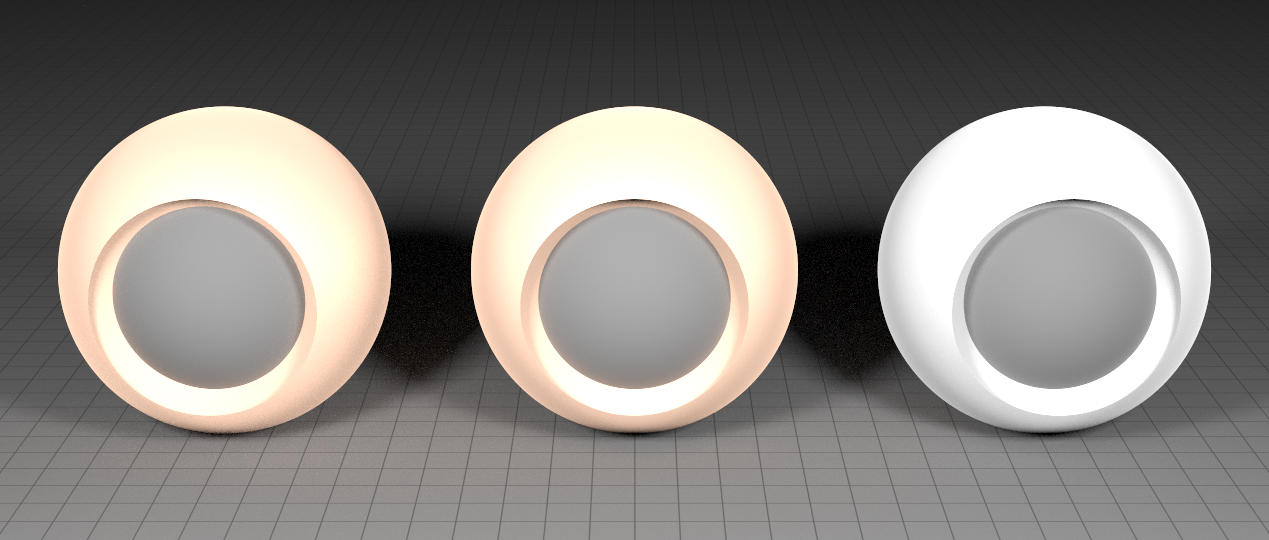
\includegraphics[scale=0.1]{img/obj/metals_al/metals_al_disney_dg1.jpg}
    \end{minipage}
    \\ \hline
  \end{tabular}
  \caption{\textit{metals\_al}}\label{tbl:myLboro}
\end{table}


\begin{table}[ht]
  \centering
  \begin{tabular}{ | c | c | c |}
    \hline
    path & const 0.6 gamma 2 & const 0.3 gamma 2 \\ \hline
    \begin{minipage}{.3\textwidth}
      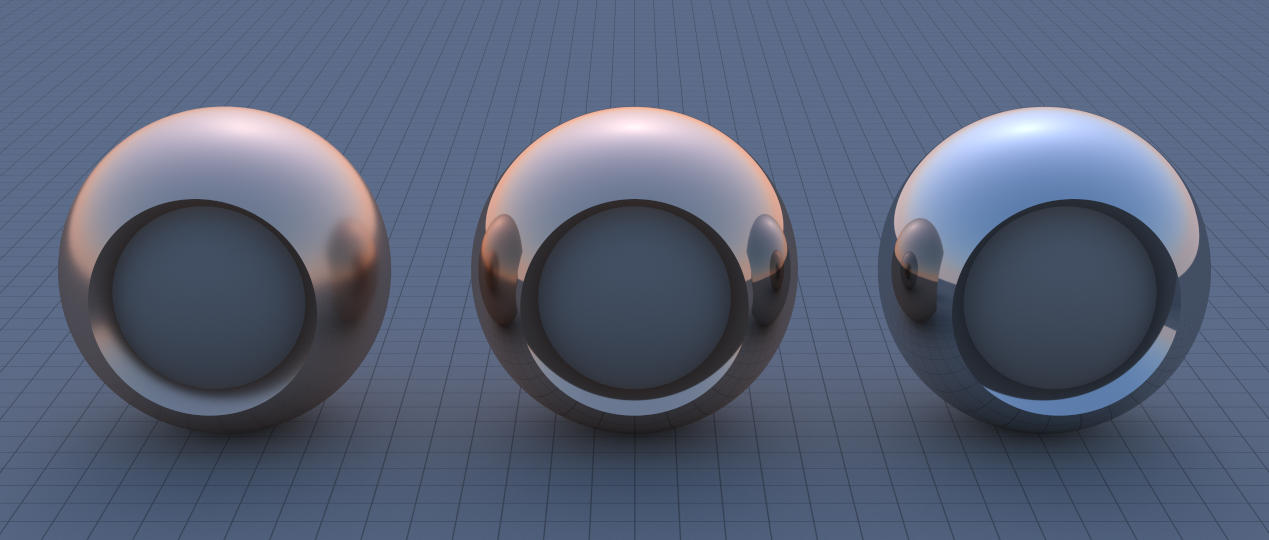
\includegraphics[scale=0.1]{img/obj/metals_el/metals_el.jpg}
    \end{minipage}
    &
    \begin{minipage}{.3\textwidth}
      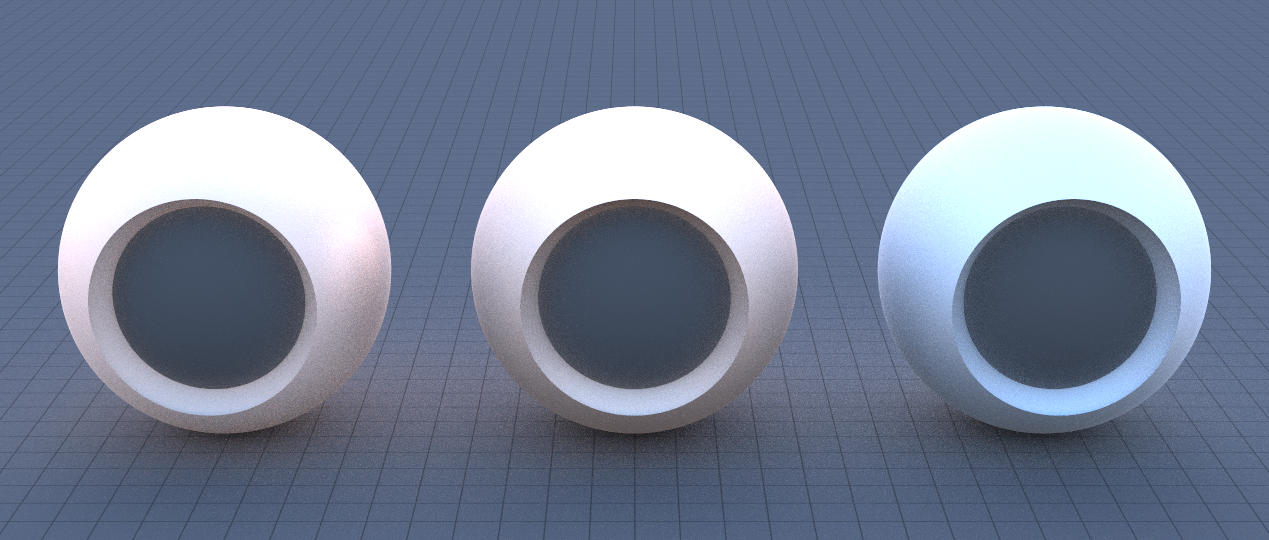
\includegraphics[scale=0.1]{img/obj/metals_el/metals_el_disney.jpg}
    \end{minipage}
    & 
    \begin{minipage}{.3\textwidth}
      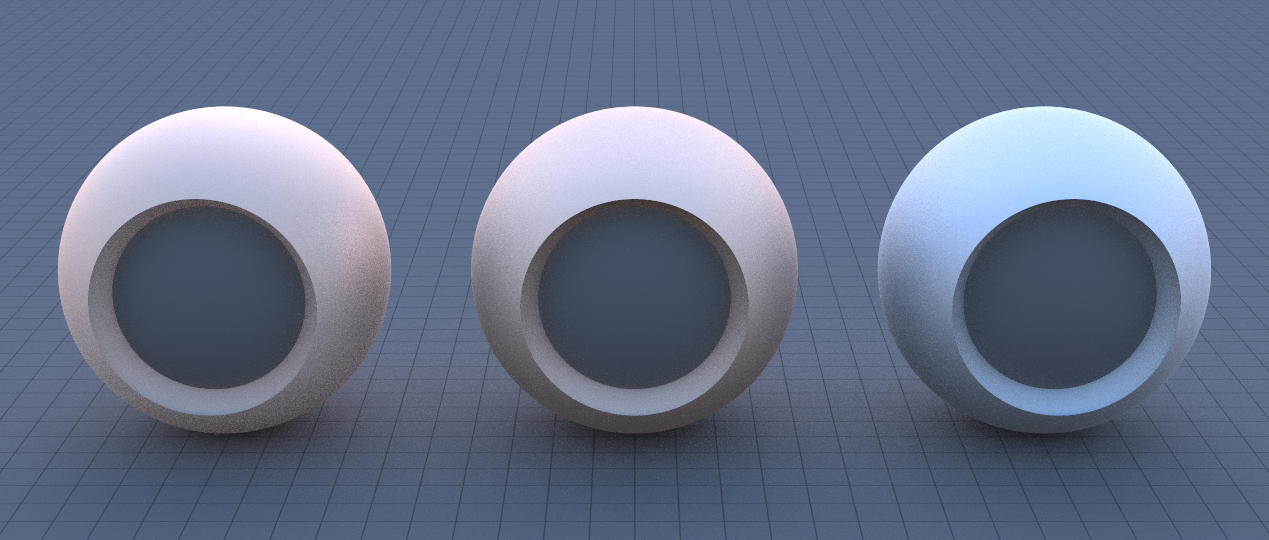
\includegraphics[scale=0.1]{img/obj/metals_el/metals_el_disney_dc03.jpg}
    \end{minipage}
    \\ \hline
  \end{tabular}
\end{table}
\begin{table}[ht]
  \centering
  \begin{tabular}{ | c | c | }
    \hline
    const 0.6 gamma 1 & const 0.3 gamma 1 \\ \hline
    \begin{minipage}{.3\textwidth}
      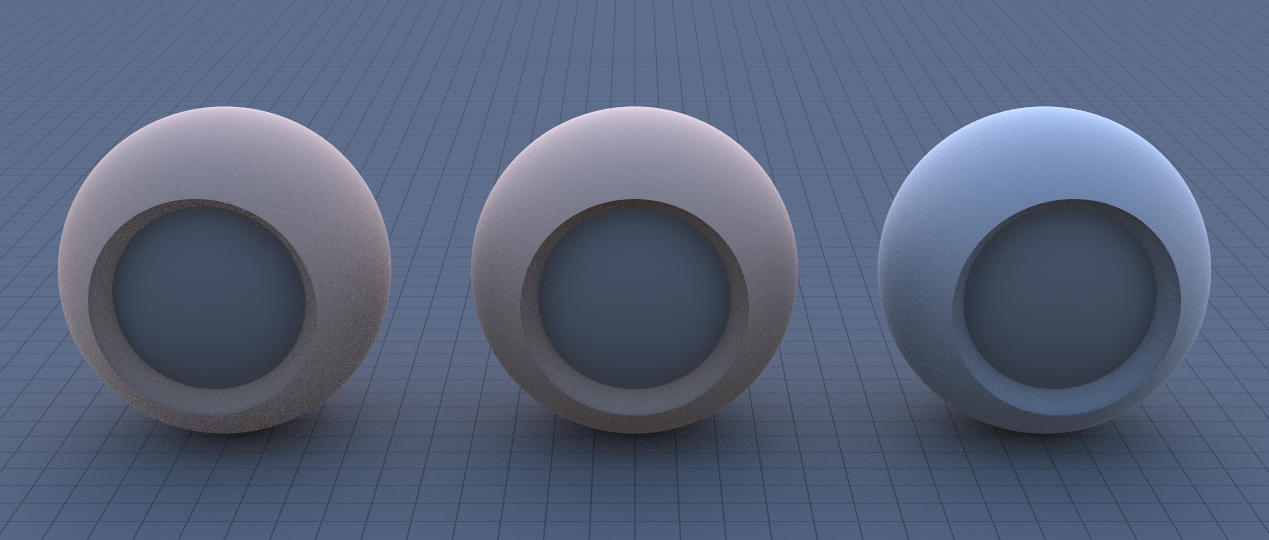
\includegraphics[scale=0.1]{img/obj/metals_el/metals_el_disney_dc03_dg1.jpg}
    \end{minipage}
    &
    \begin{minipage}{.3\textwidth}
      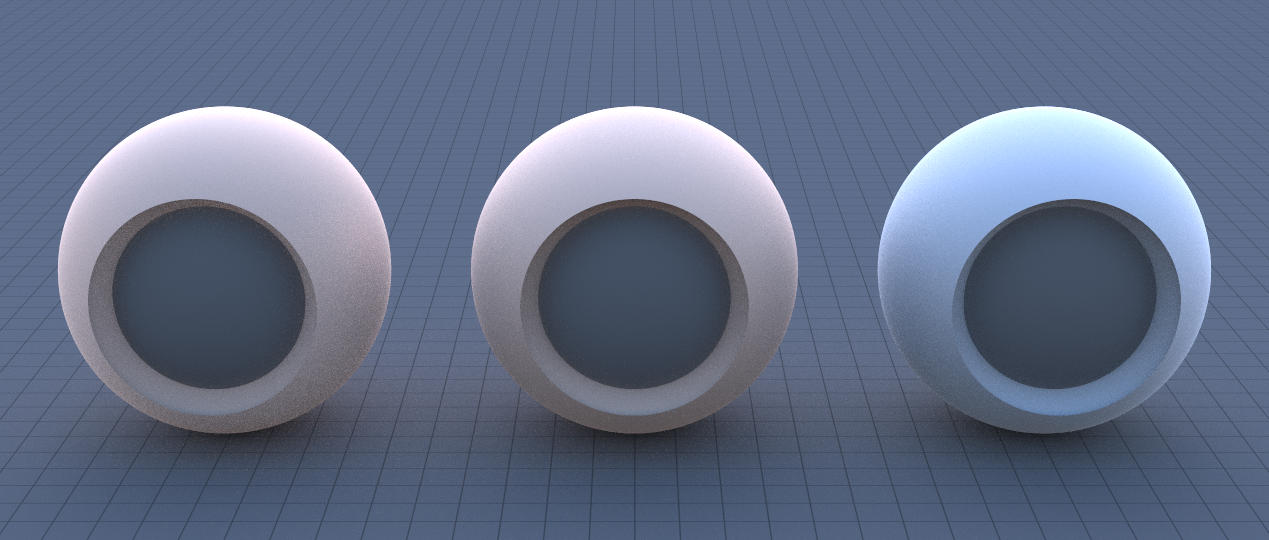
\includegraphics[scale=0.1]{img/obj/metals_el/metals_el_disney_dg1.jpg}
    \end{minipage}
    \\ \hline
  \end{tabular}
  \caption{\textit{metals\_pl}}\label{tbl:myLboro}
\end{table}


\begin{table}[ht]
  \centering
  \begin{tabular}{ | c | c | c |}
    \hline
    path & const 0.6 gamma 2 & const 0.3 gamma 2 \\ \hline
    \begin{minipage}{.3\textwidth}
      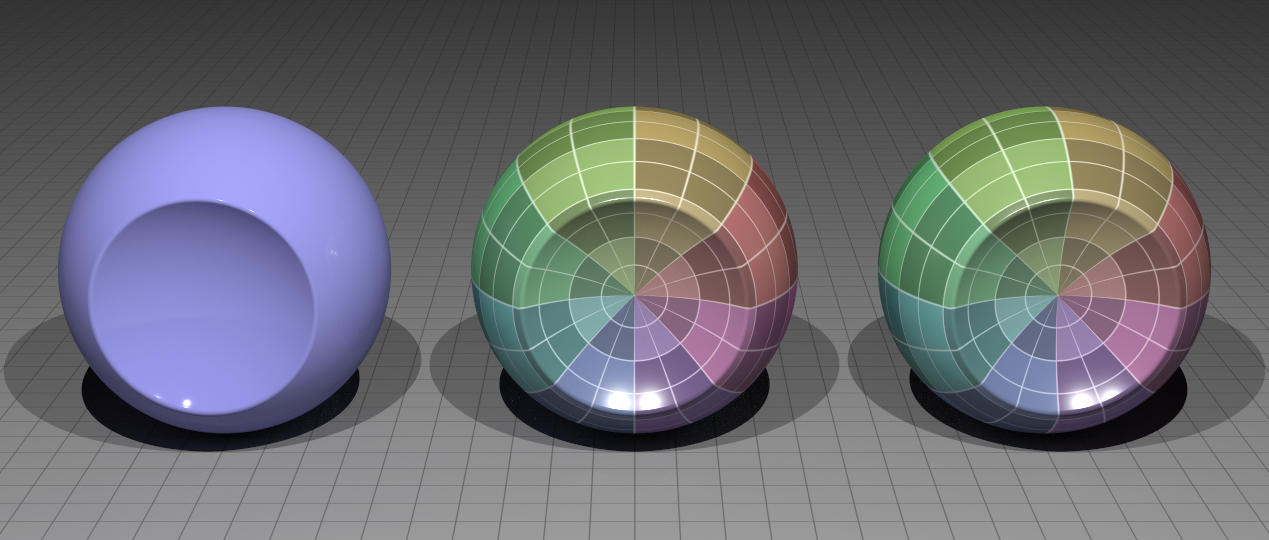
\includegraphics[scale=0.1]{img/obj/normalmap_pl/normalmap_pl.jpg}
    \end{minipage}
    &
    \begin{minipage}{.3\textwidth}
      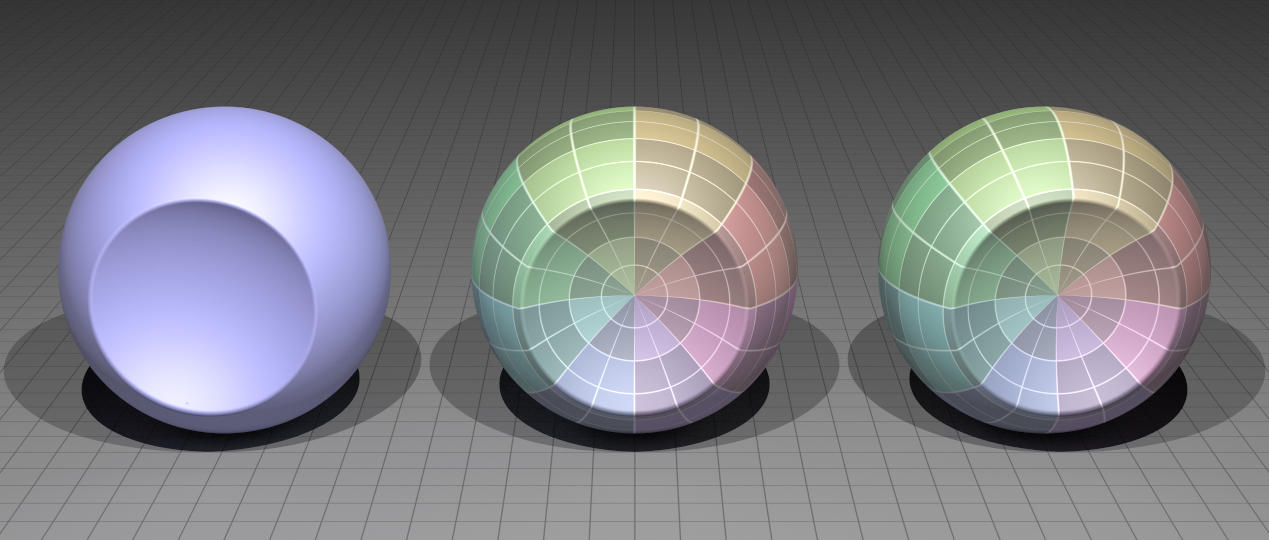
\includegraphics[scale=0.1]{img/obj/normalmap_pl/normalmap_pl_disney.jpg}
    \end{minipage}
    & 
    \begin{minipage}{.3\textwidth}
      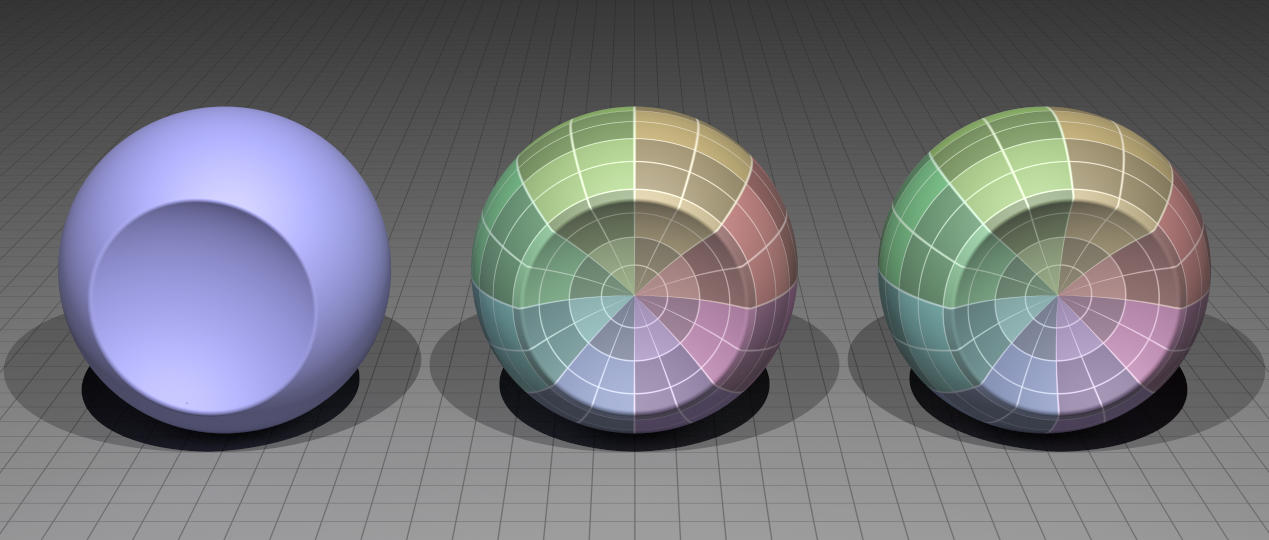
\includegraphics[scale=0.1]{img/obj/normalmap_pl/normalmap_pl_disney_dc03.jpg}
    \end{minipage}
    \\ \hline
  \end{tabular}
\end{table}
\begin{table}[ht]
  \centering
  \begin{tabular}{ | c | c | }
    \hline
    const 0.6 gamma 1 & const 0.3 gamma 1 \\ \hline
    \begin{minipage}{.3\textwidth}
      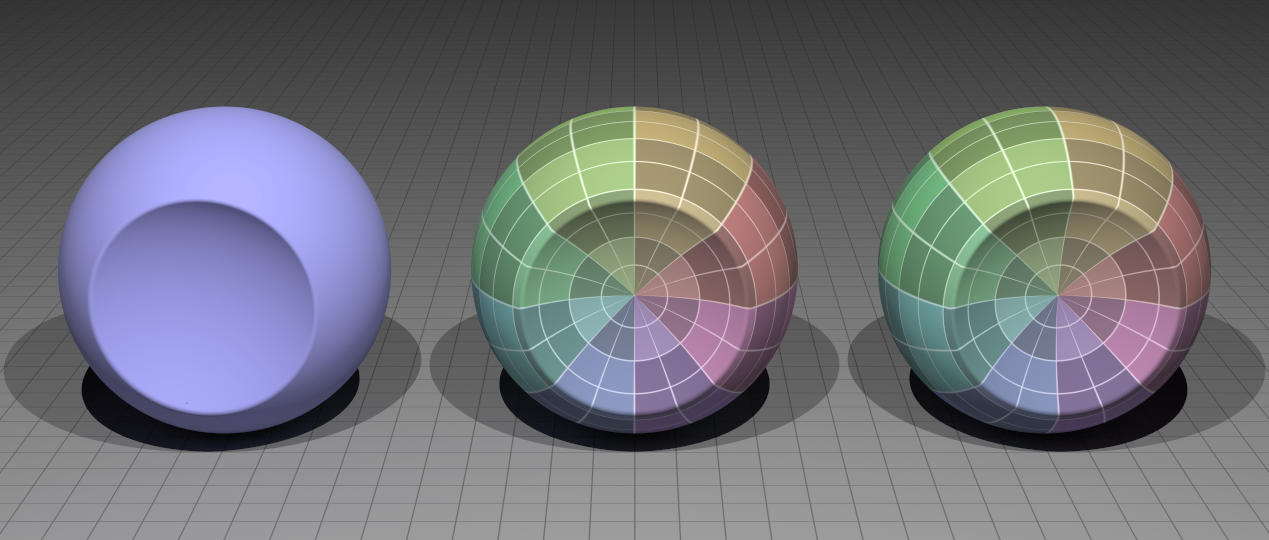
\includegraphics[scale=0.1]{img/obj/normalmap_pl/normalmap_pl_disney_dc03_dg1.jpg}
    \end{minipage}
    &
    \begin{minipage}{.3\textwidth}
      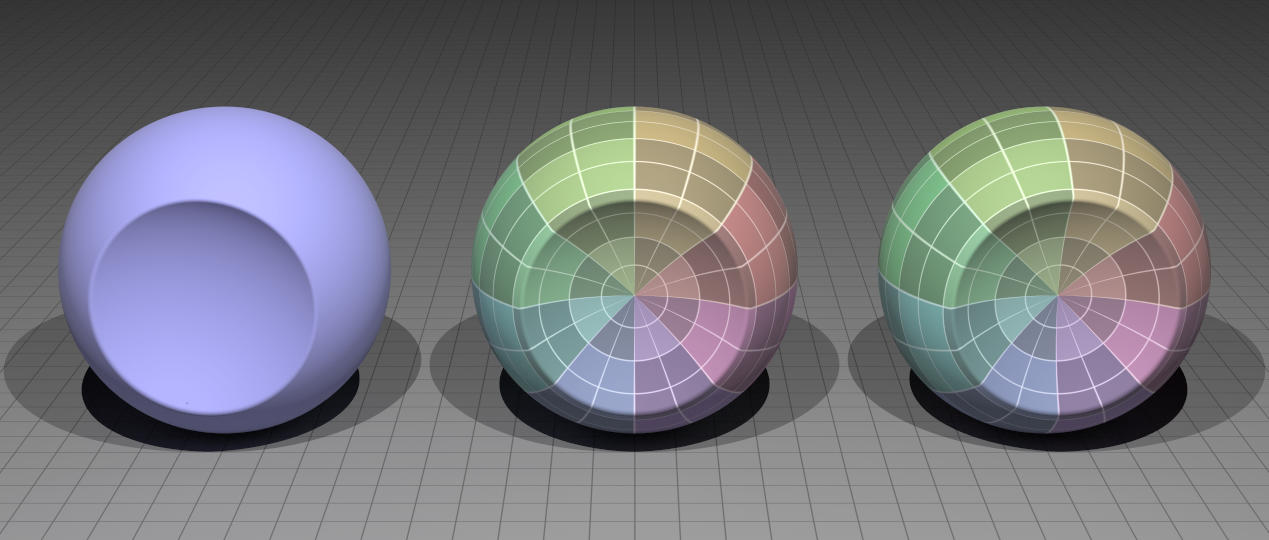
\includegraphics[scale=0.1]{img/obj/normalmap_pl/normalmap_pl_disney_dg1.jpg}
    \end{minipage}
    \\ \hline
  \end{tabular}
  \caption{\textit{normalmap\_pl}}\label{tbl:myLboro}
\end{table}


\begin{table}[ht]
  \centering
  \begin{tabular}{ | c | c | c |}
    \hline
    path & const 0.6 gamma 2 & const 0.3 gamma 2 \\ \hline
    \begin{minipage}{.3\textwidth}
      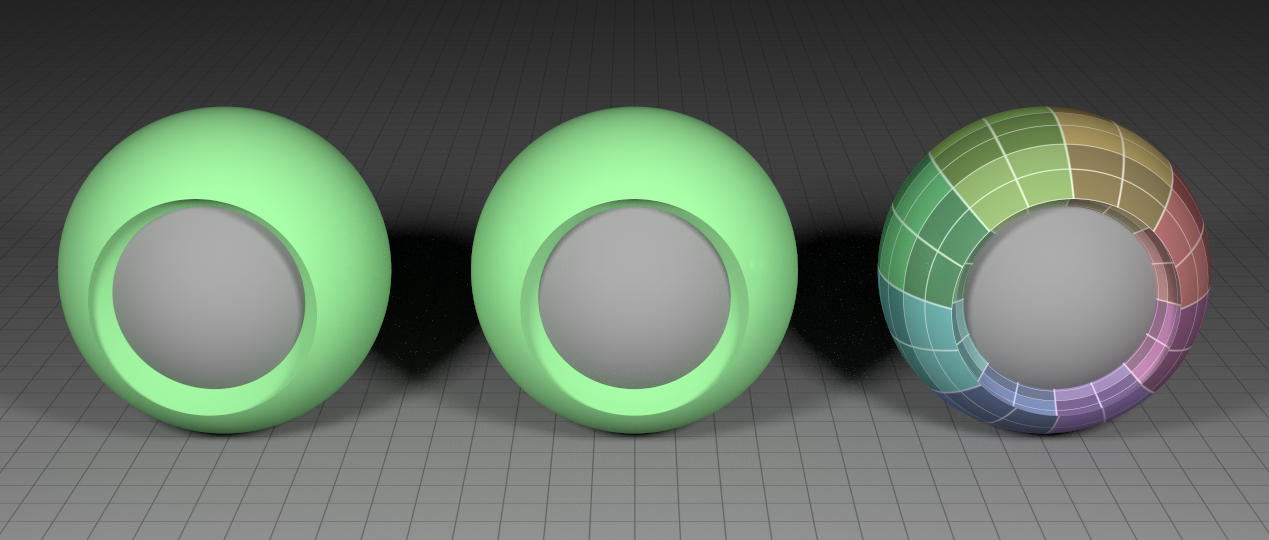
\includegraphics[scale=0.1]{img/obj/plastics_al/plastics_al.jpg}
    \end{minipage}
    &
    \begin{minipage}{.3\textwidth}
      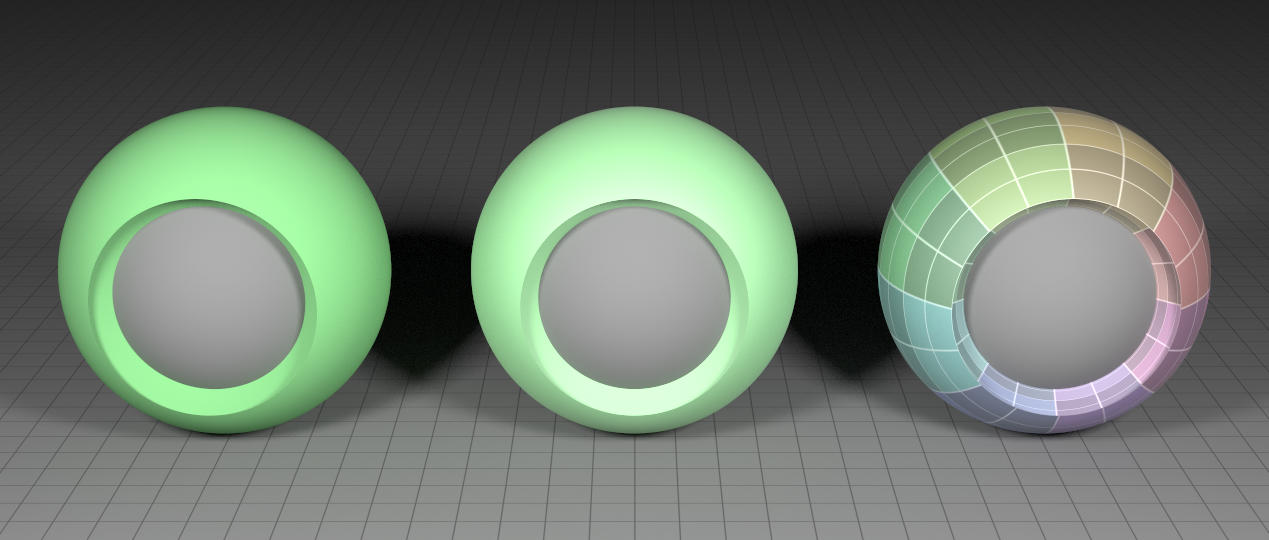
\includegraphics[scale=0.1]{img/obj/plastics_al/plastics_al_disney.jpg}
    \end{minipage}
    & 
    \begin{minipage}{.3\textwidth}
      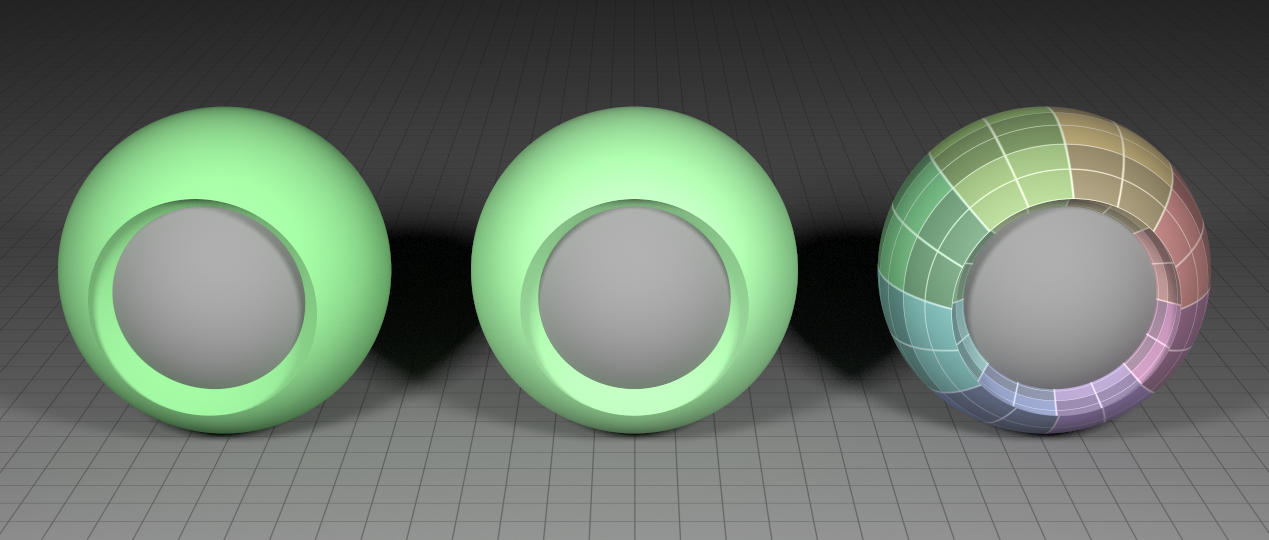
\includegraphics[scale=0.1]{img/obj/plastics_al/plastics_al_disney_dc03.jpg}
    \end{minipage}
    \\ \hline
  \end{tabular}
\end{table}
\begin{table}[ht]
  \centering
  \begin{tabular}{ | c | c | }
    \hline
    const 0.6 gamma 1 & const 0.3 gamma 1 \\ \hline
    \begin{minipage}{.3\textwidth}
      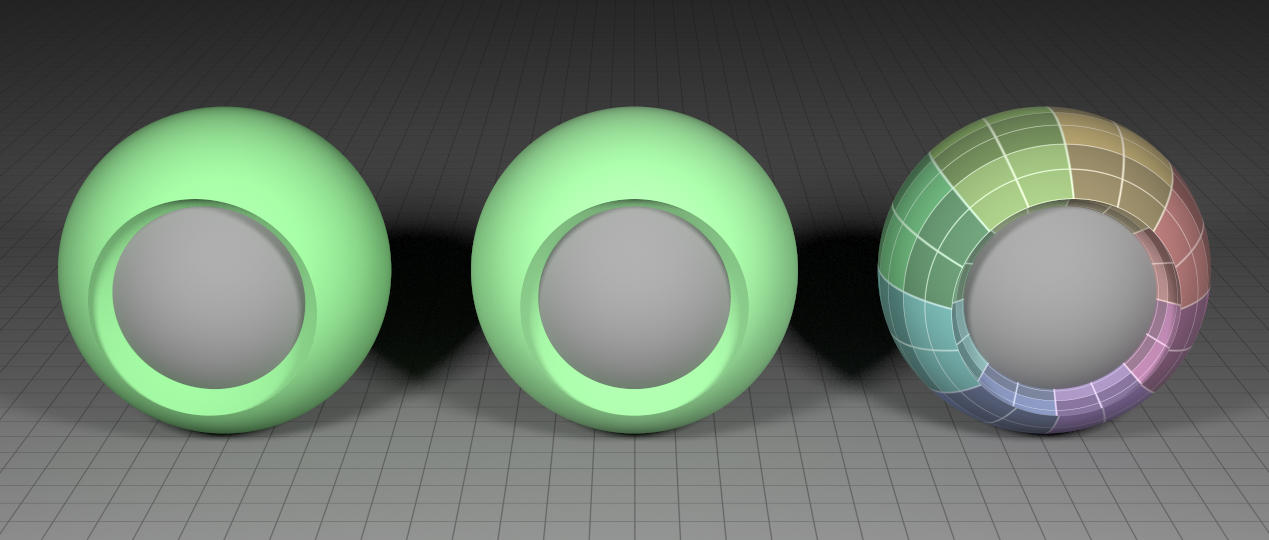
\includegraphics[scale=0.1]{img/obj/plastics_al/plastics_al_disney_dc03_dg1.jpg}
    \end{minipage}
    &
    \begin{minipage}{.3\textwidth}
      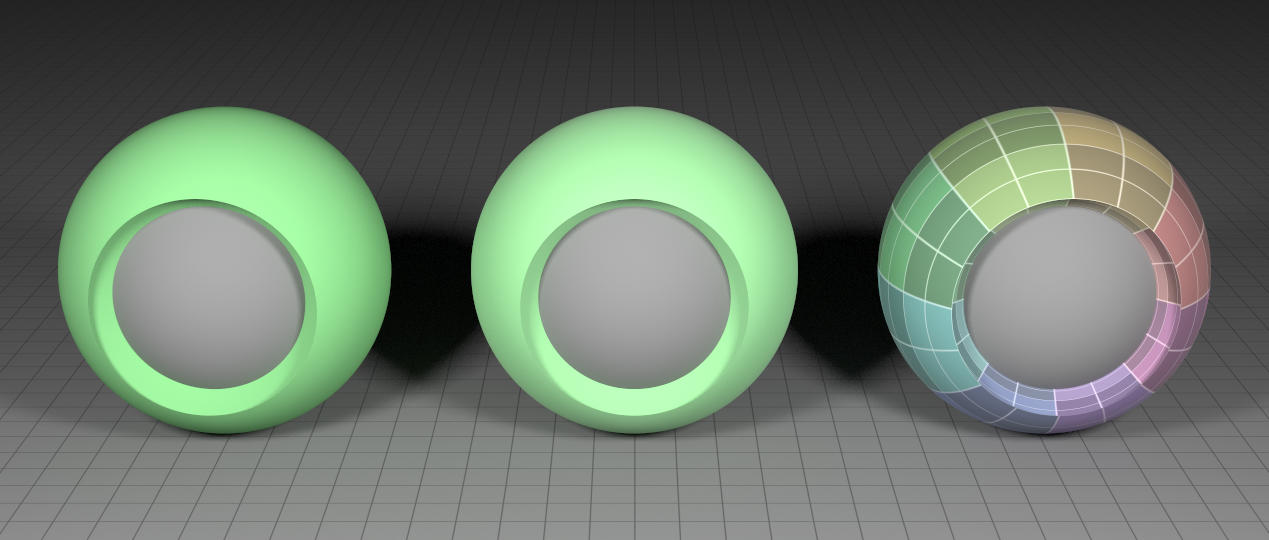
\includegraphics[scale=0.1]{img/obj/plastics_al/plastics_al_disney_dg1.jpg}
    \end{minipage}
    \\ \hline
  \end{tabular}
  \caption{\textit{plastics\_al}}\label{tbl:myLboro}
\end{table}


\begin{table}[ht]
  \centering
  \begin{tabular}{ | c | c | c |}
    \hline
    path & const 0.6 gamma 2 & const 0.3 gamma 2 \\ \hline
    \begin{minipage}{.3\textwidth}
      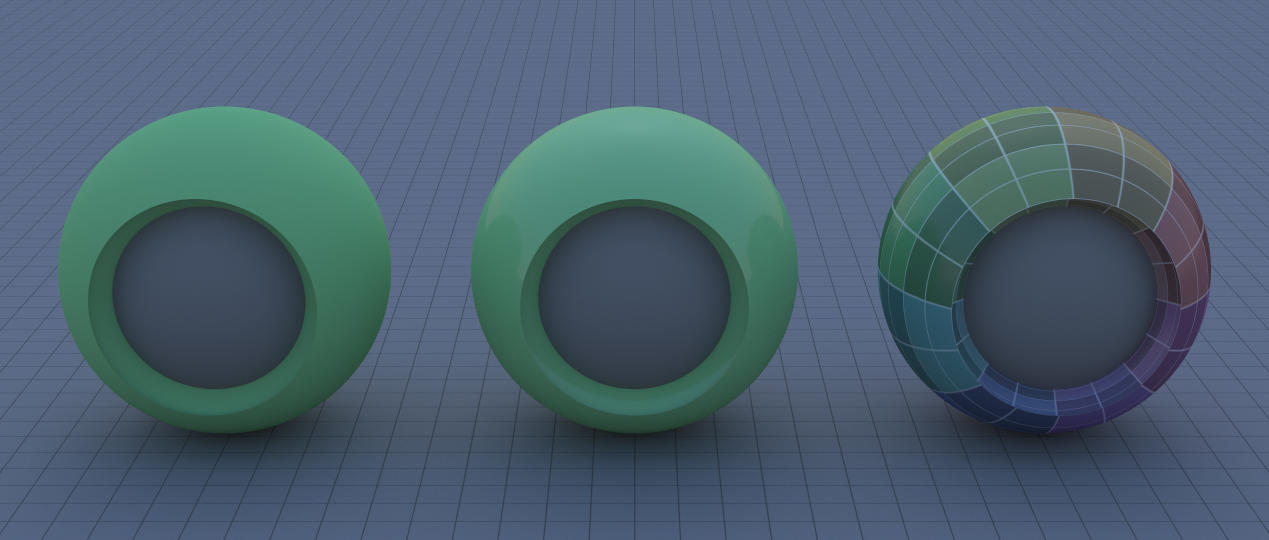
\includegraphics[scale=0.1]{img/obj/plastics_el/plastics_el.jpg}
    \end{minipage}
    &
    \begin{minipage}{.3\textwidth}
      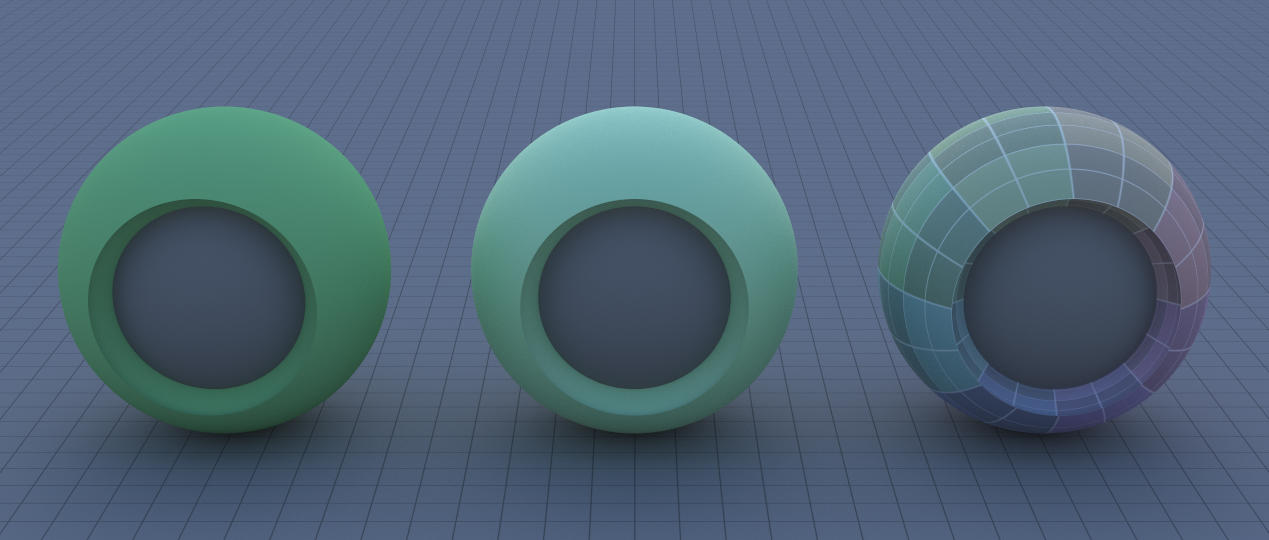
\includegraphics[scale=0.1]{img/obj/plastics_el/plastics_el_disney.jpg}
    \end{minipage}
    & 
    \begin{minipage}{.3\textwidth}
      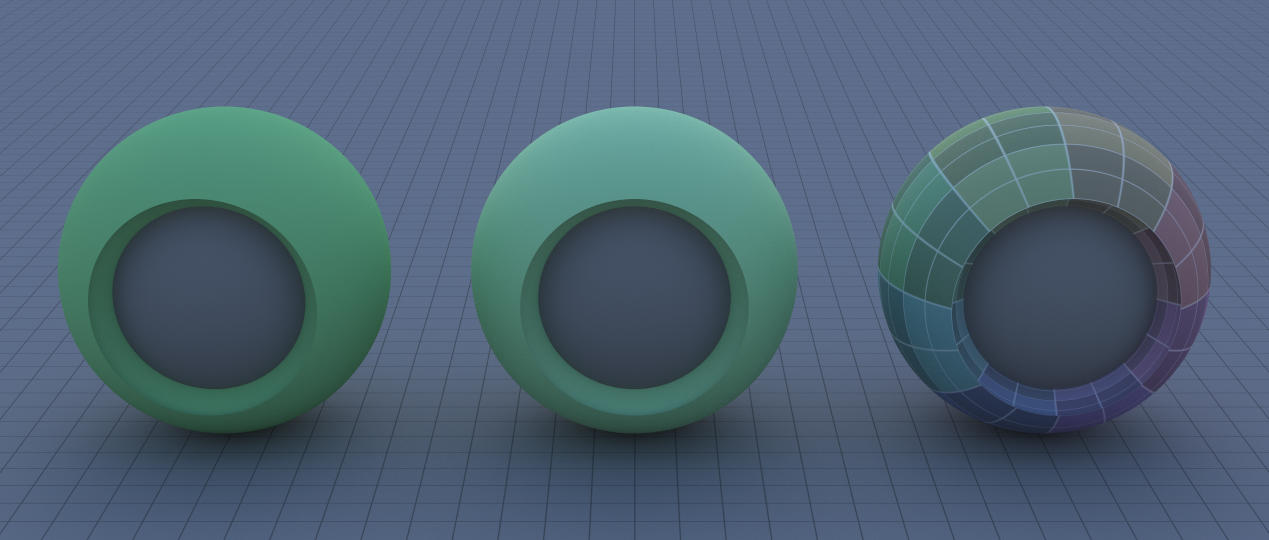
\includegraphics[scale=0.1]{img/obj/plastics_el/plastics_el_disney_dc03.jpg}
    \end{minipage}
    \\ \hline
  \end{tabular}
\end{table}
\begin{table}[ht]
  \centering
  \begin{tabular}{ | c | c | }
    \hline
    const 0.6 gamma 1 & const 0.3 gamma 1 \\ \hline
    \begin{minipage}{.3\textwidth}
      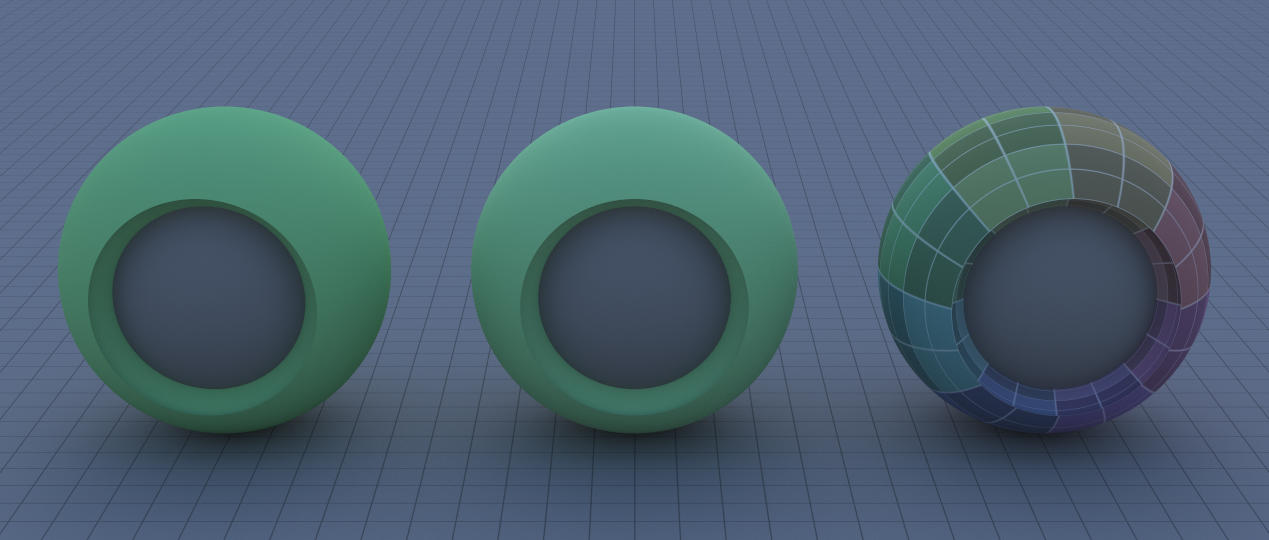
\includegraphics[scale=0.1]{img/obj/plastics_el/plastics_el_disney_dc03_dg1.jpg}
    \end{minipage}
    &
    \begin{minipage}{.3\textwidth}
      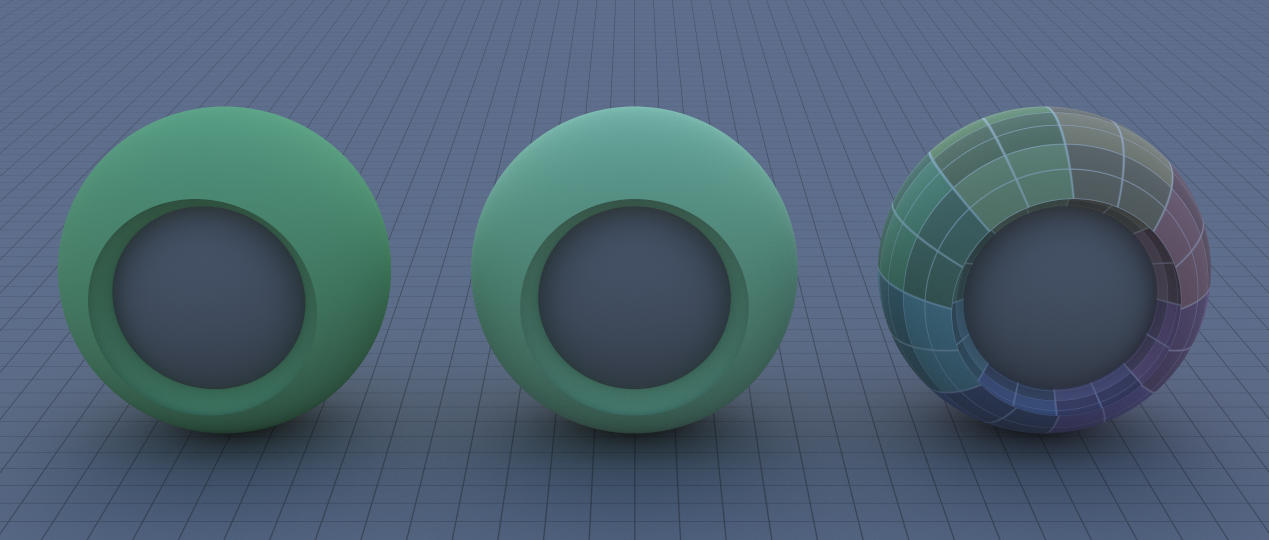
\includegraphics[scale=0.1]{img/obj/plastics_el/plastics_el_disney_dg1.jpg}
    \end{minipage}
    \\ \hline
  \end{tabular}
  \caption{\textit{plastics\_el}}\label{tbl:myLboro}
\end{table}


\begin{table}[ht]
  \centering
  \begin{tabular}{ | c | c | c |}
    \hline
    path & const 0.6 gamma 2 & const 0.3 gamma 2 \\ \hline
    \begin{minipage}{.3\textwidth}
      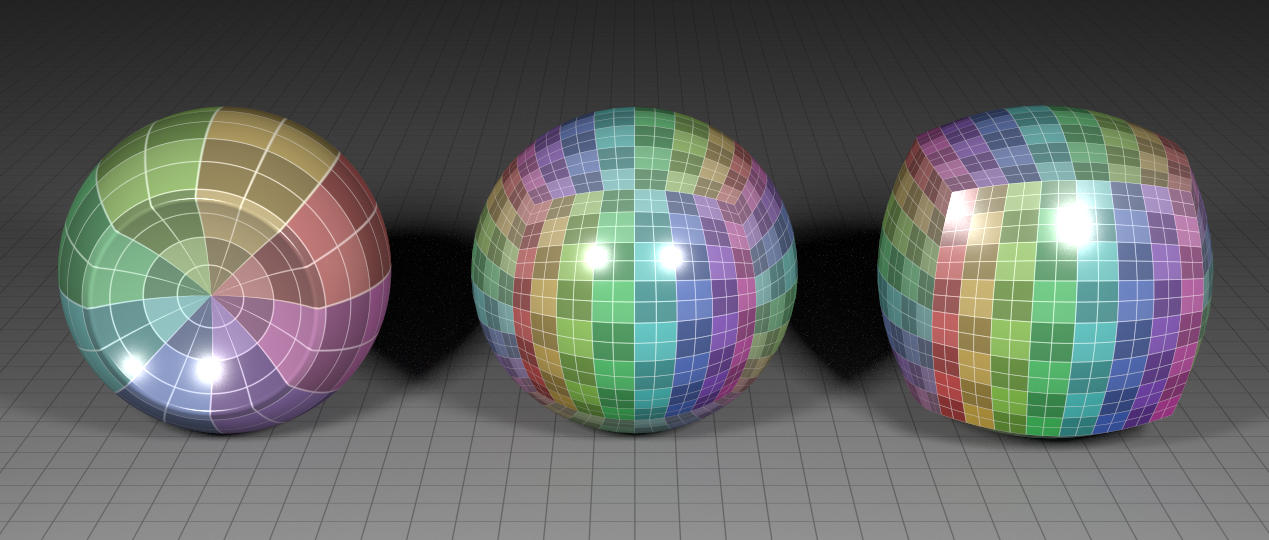
\includegraphics[scale=0.1]{img/obj/simple_al/simple_al.jpg}
    \end{minipage}
    &
    \begin{minipage}{.3\textwidth}
      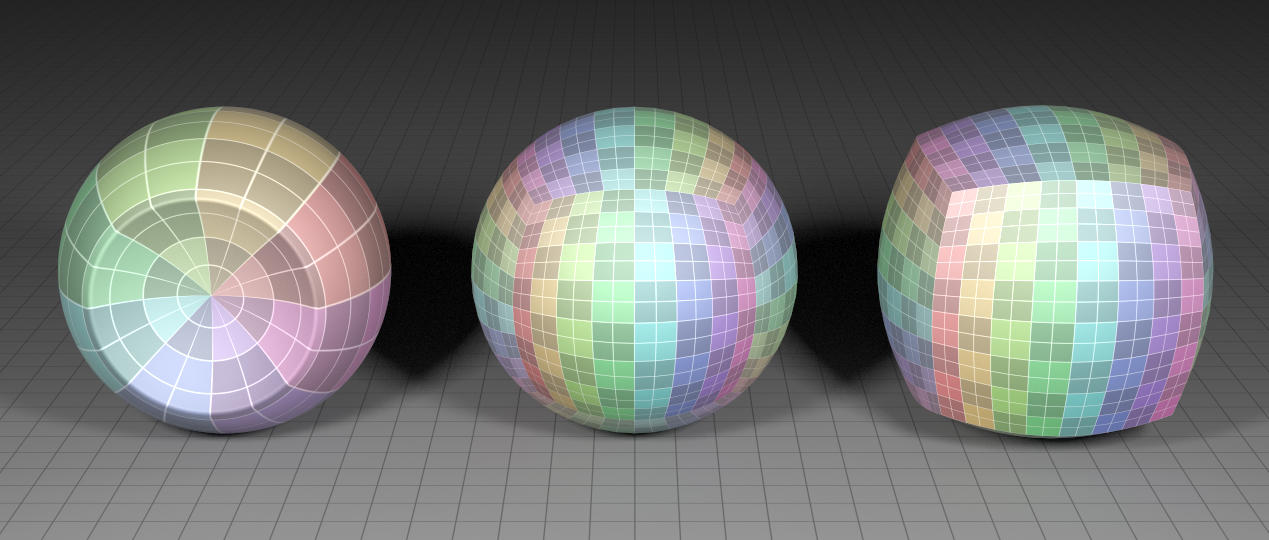
\includegraphics[scale=0.1]{img/obj/simple_al/simple_al_disney.jpg}
    \end{minipage}
    & 
    \begin{minipage}{.3\textwidth}
      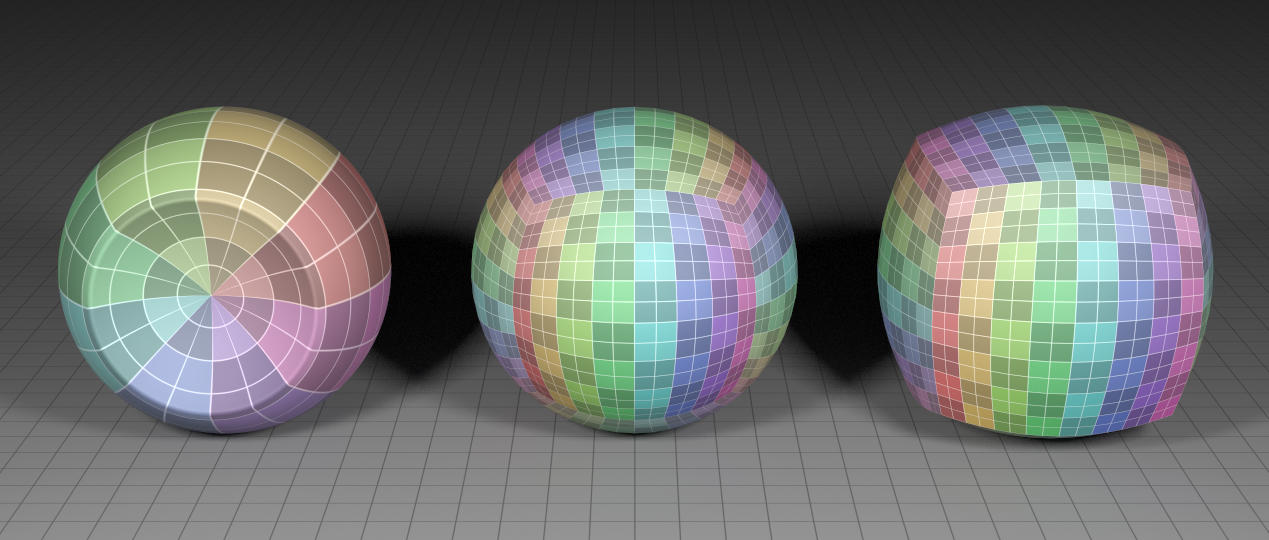
\includegraphics[scale=0.1]{img/obj/simple_al/simple_al_disney_dc03.jpg}
    \end{minipage}
    \\ \hline
  \end{tabular}
\end{table}
\begin{table}[ht]
  \centering
  \begin{tabular}{ | c | c | }
    \hline
    const 0.6 gamma 1 & const 0.3 gamma 1 \\ \hline
    \begin{minipage}{.3\textwidth}
      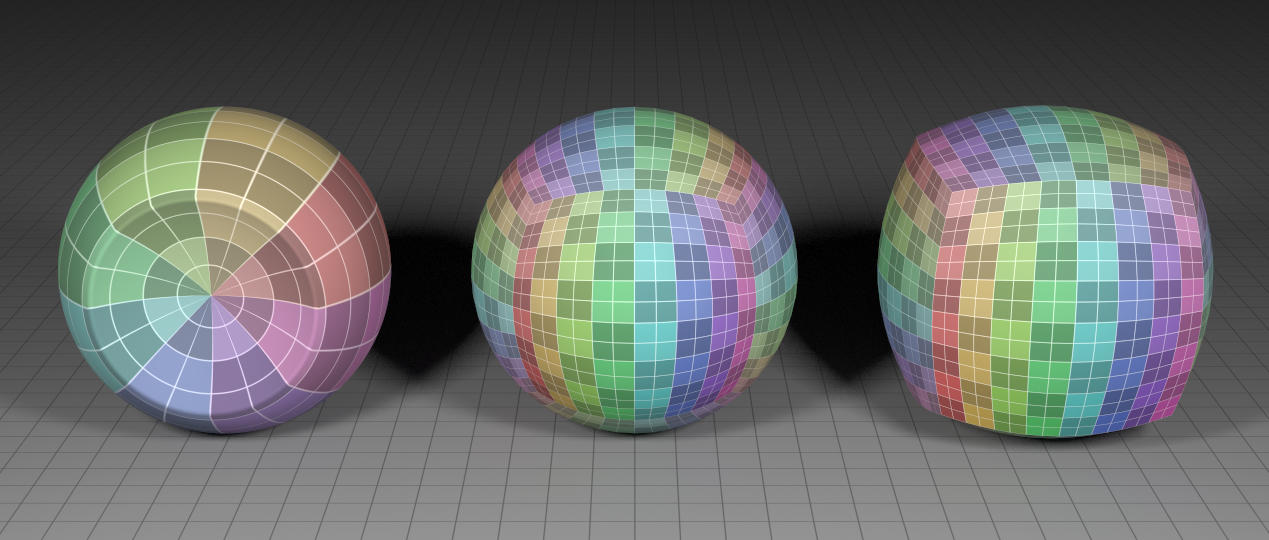
\includegraphics[scale=0.1]{img/obj/simple_al/simple_al_disney_dc03_dg1.jpg}
    \end{minipage}
    &
    \begin{minipage}{.3\textwidth}
      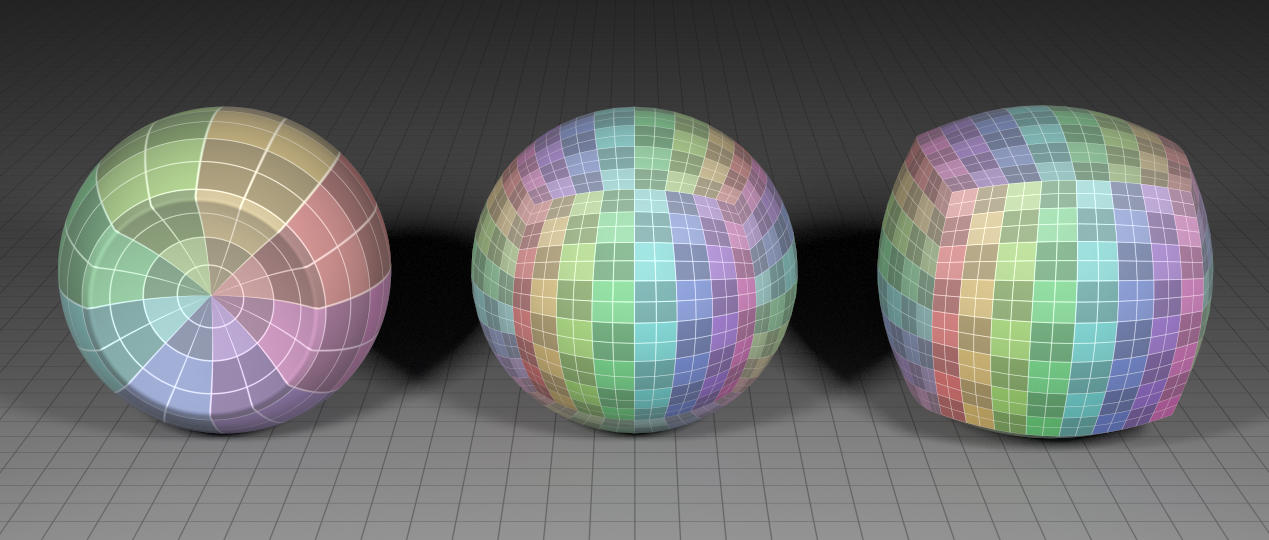
\includegraphics[scale=0.1]{img/obj/simple_al/simple_al_disney_dg1.jpg}
    \end{minipage}
    \\ \hline
  \end{tabular}
  \caption{\textit{simple\_al}}\label{tbl:myLboro}
\end{table}


\begin{table}[ht]
  \centering
  \begin{tabular}{ | c | c | c |}
    \hline
    path & const 0.6 gamma 2 & const 0.3 gamma 2 \\ \hline
    \begin{minipage}{.3\textwidth}
      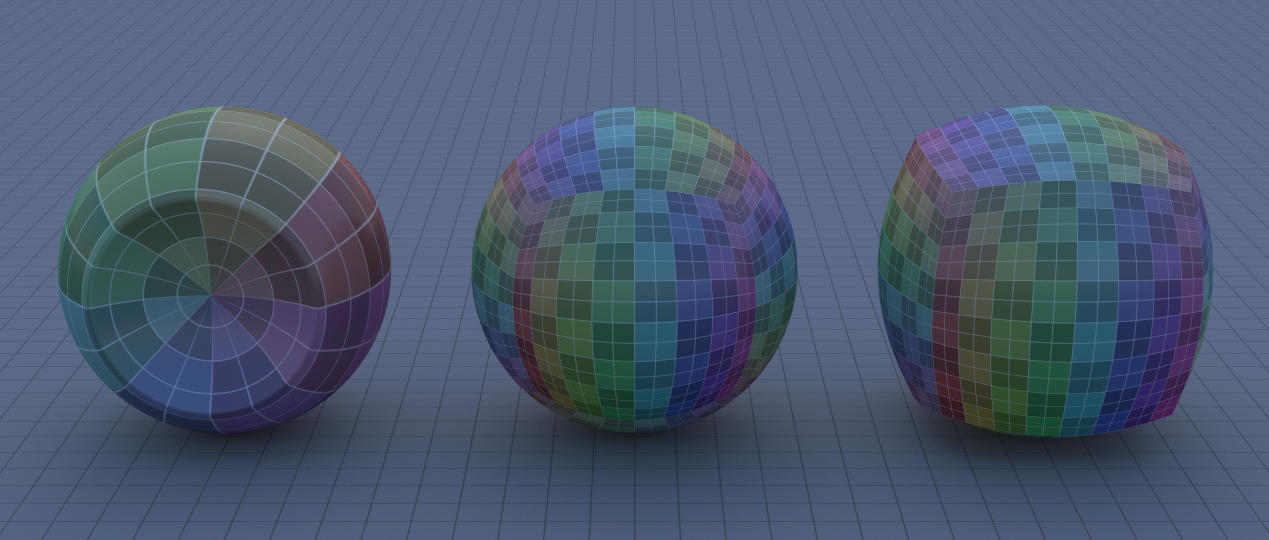
\includegraphics[scale=0.1]{img/obj/simple_el/simple_el.jpg}
    \end{minipage}
    &
    \begin{minipage}{.3\textwidth}
      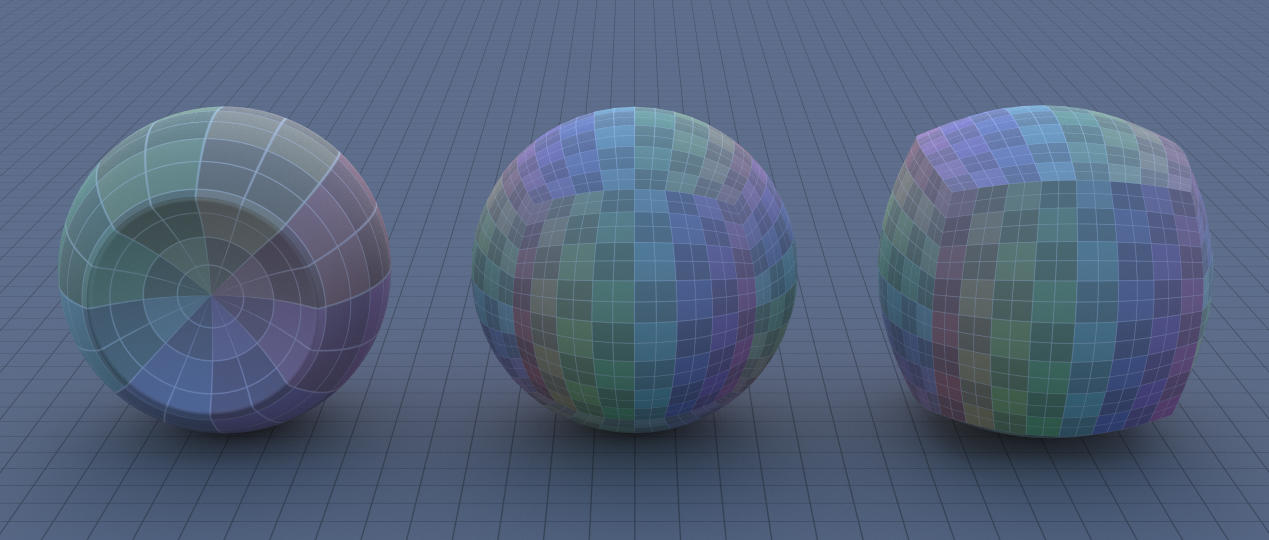
\includegraphics[scale=0.1]{img/obj/simple_el/simple_el_disney.jpg}
    \end{minipage}
    & 
    \begin{minipage}{.3\textwidth}
      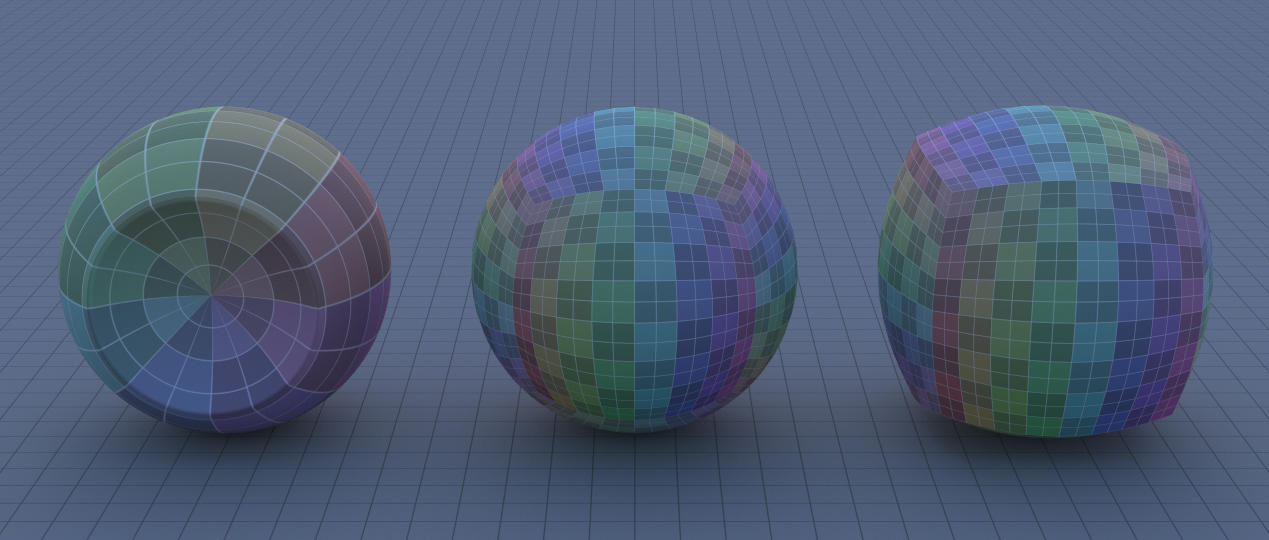
\includegraphics[scale=0.1]{img/obj/simple_el/simple_el_disney_dc03.jpg}
    \end{minipage}
    \\ \hline
  \end{tabular}
\end{table}
\begin{table}[ht]
  \centering
  \begin{tabular}{ | c | c | }
    \hline
    const 0.6 gamma 1 & const 0.3 gamma 1 \\ \hline
    \begin{minipage}{.3\textwidth}
      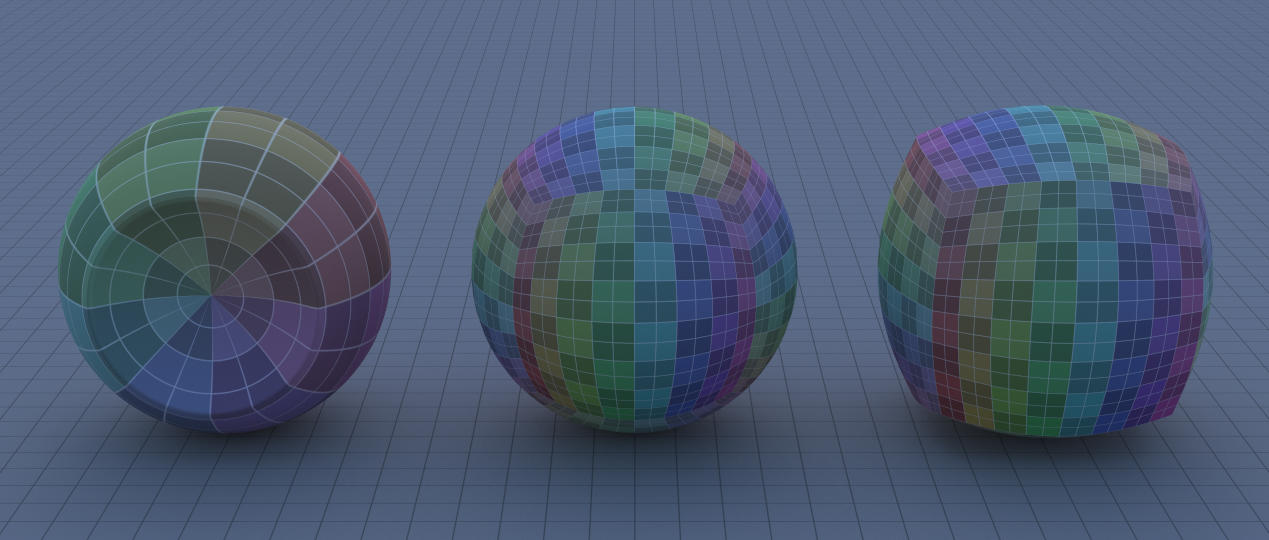
\includegraphics[scale=0.1]{img/obj/simple_el/simple_el_disney_dc03_dg1.jpg}
    \end{minipage}
    &
    \begin{minipage}{.3\textwidth}
      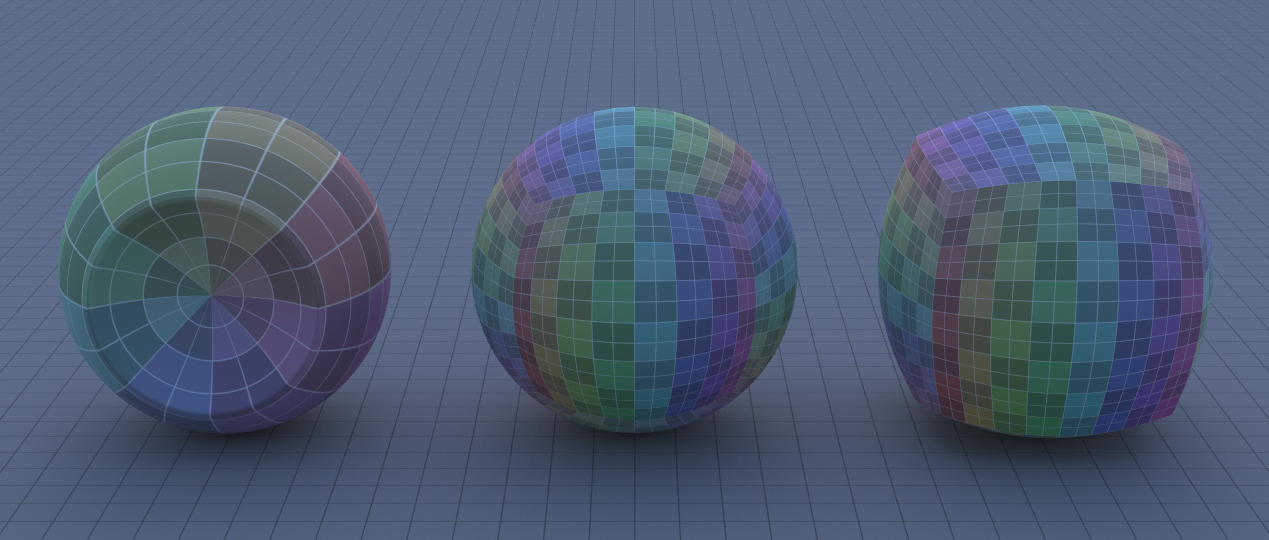
\includegraphics[scale=0.1]{img/obj/simple_el/simple_el_disney_dg1.jpg}
    \end{minipage}
    \\ \hline
  \end{tabular}
  \caption{\textit{simple\_el}}\label{tbl:myLboro}
\end{table}


\begin{table}[ht]
  \centering
  \begin{tabular}{ | c | c | c |}
    \hline
    path & const 0.6 gamma 2 & const 0.3 gamma 2 \\ \hline
    \begin{minipage}{.3\textwidth}
      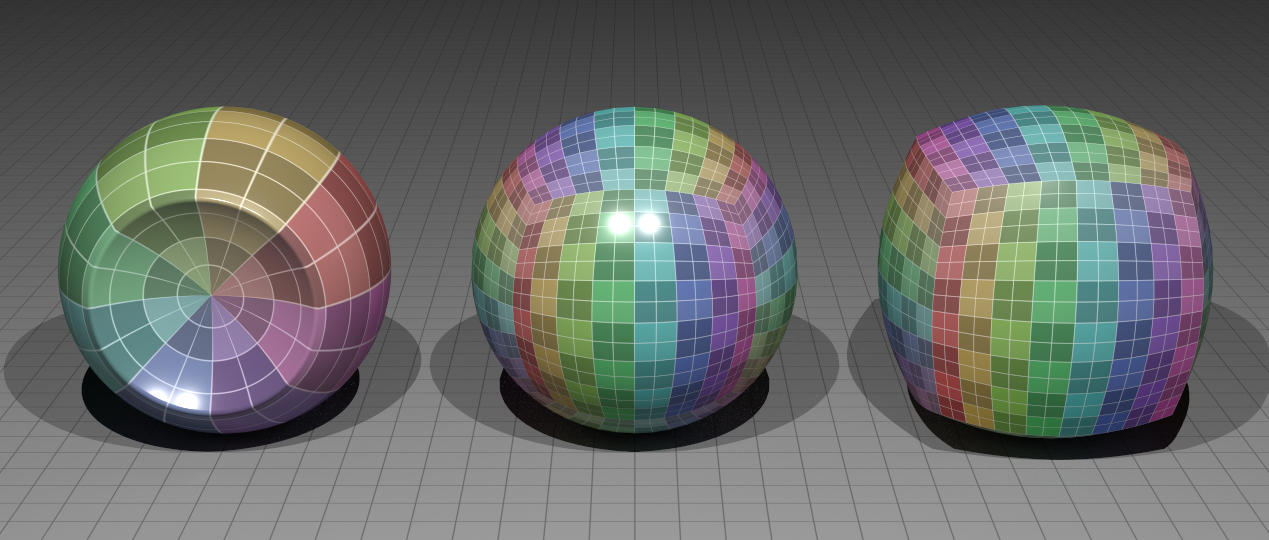
\includegraphics[scale=0.1]{img/obj/simple_pl/simple_pl.jpg}
    \end{minipage}
    &
    \begin{minipage}{.3\textwidth}
      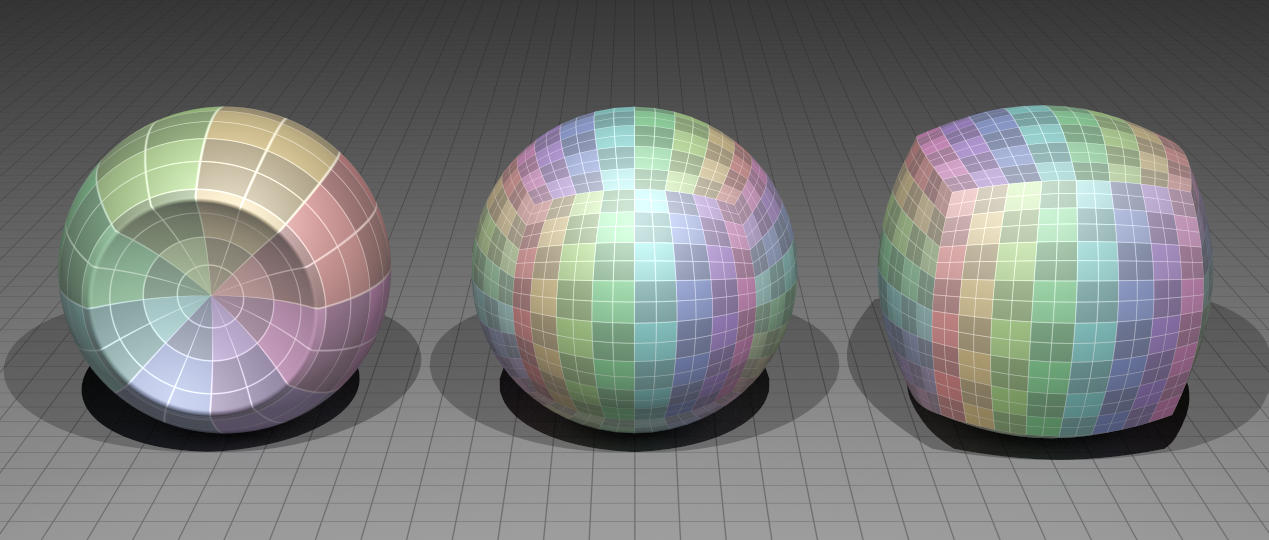
\includegraphics[scale=0.1]{img/obj/simple_pl/simple_pl_disney.jpg}
    \end{minipage}
    & 
    \begin{minipage}{.3\textwidth}
      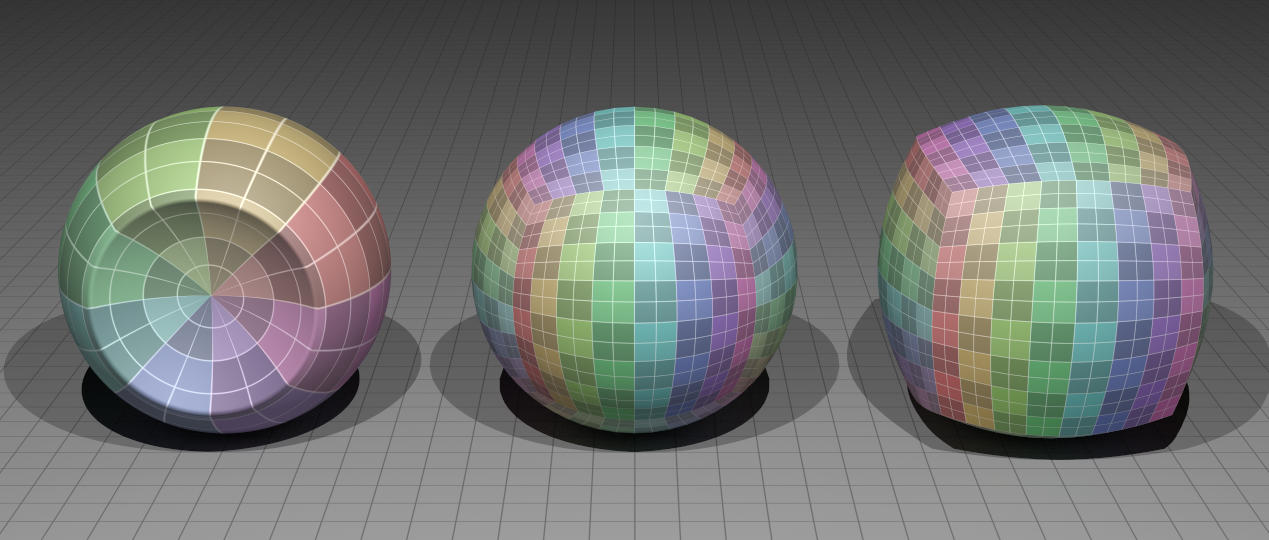
\includegraphics[scale=0.1]{img/obj/simple_pl/simple_pl_disney_dc03.jpg}
    \end{minipage}
    \\ \hline
  \end{tabular}
\end{table}
\begin{table}[ht]
  \centering
  \begin{tabular}{ | c | c | }
    \hline
    const 0.6 gamma 1 & const 0.3 gamma 1 \\ \hline
    \begin{minipage}{.3\textwidth}
      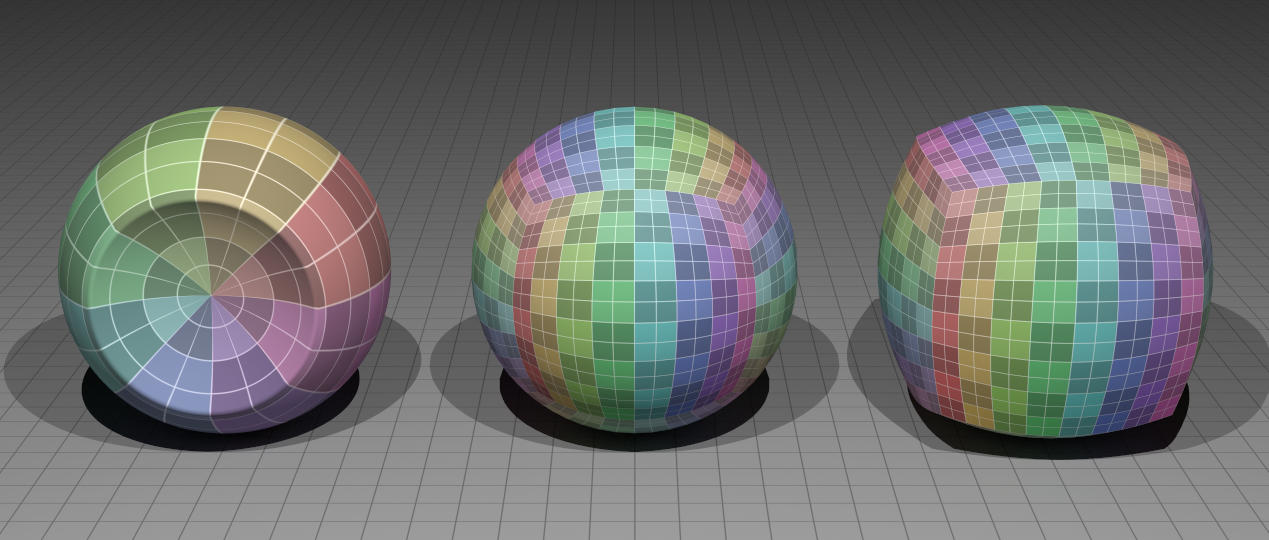
\includegraphics[scale=0.1]{img/obj/simple_pl/simple_pl_disney_dc03_dg1.jpg}
    \end{minipage}
    &
    \begin{minipage}{.3\textwidth}
      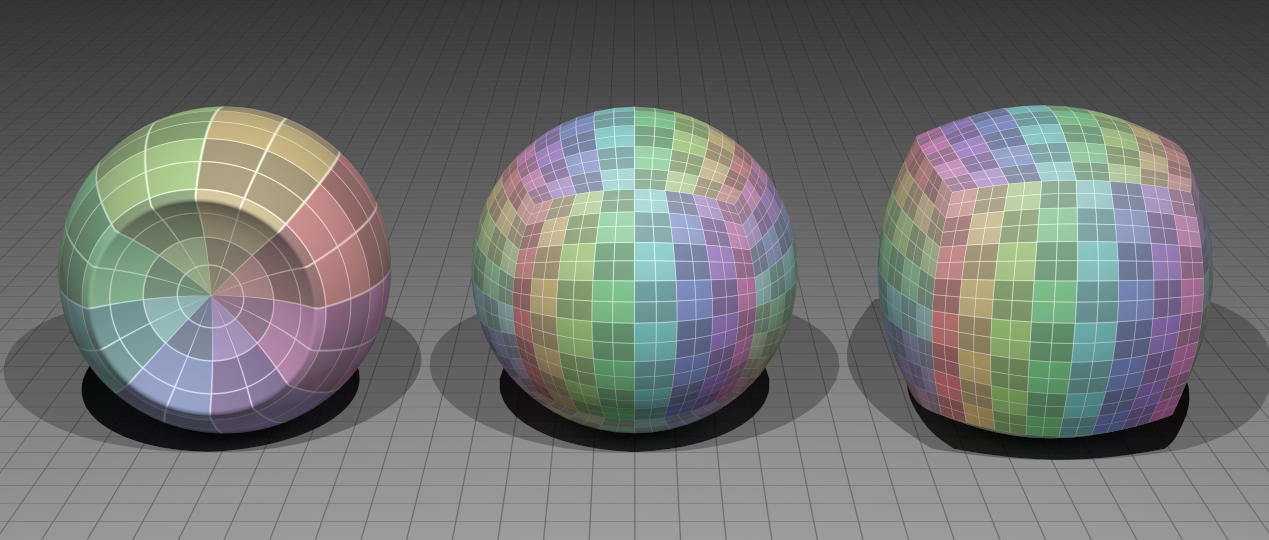
\includegraphics[scale=0.1]{img/obj/simple_pl/simple_pl_disney_dg1.jpg}
    \end{minipage}
    \\ \hline
  \end{tabular}
  \caption{\textit{simple\_pl}}\label{tbl:myLboro}
\end{table}


\begin{table}[ht]
  \centering
  \begin{tabular}{ | c | c | c |}
    \hline
    path & const 0.6 gamma 2 & const 0.3 gamma 2 \\ \hline
    \begin{minipage}{.3\textwidth}
      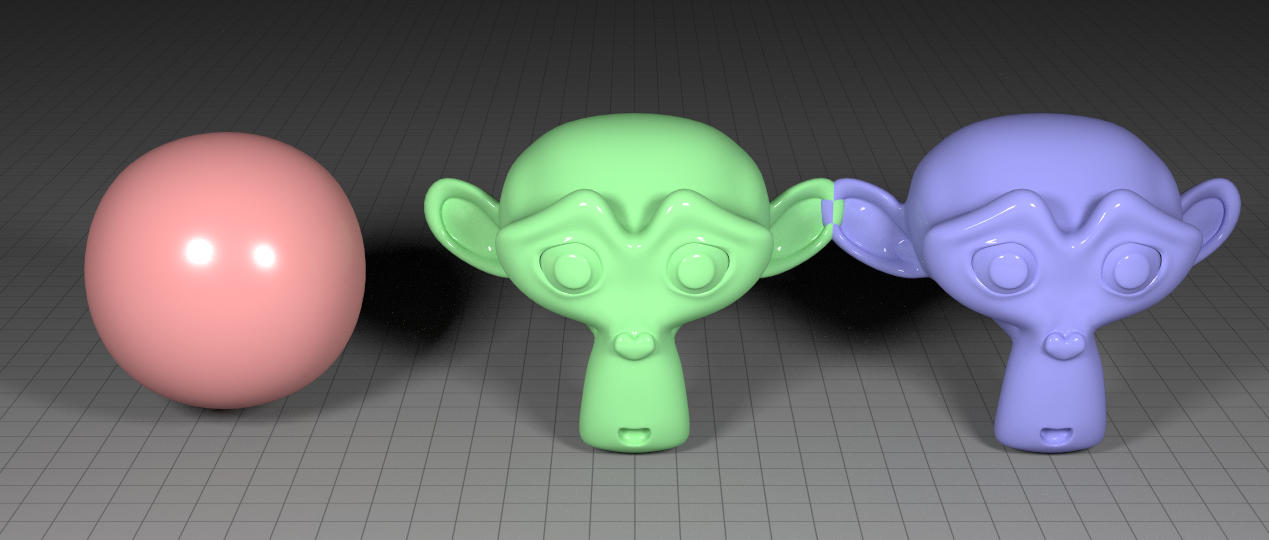
\includegraphics[scale=0.1]{img/obj/subdiv_al/subdiv_al.jpg}
    \end{minipage}
    &
    \begin{minipage}{.3\textwidth}
      \includegraphics[scale=0.1]{img/obj/subdiv_al/subdiv_al_disney.jpg}
    \end{minipage}
    & 
    \begin{minipage}{.3\textwidth}
      \includegraphics[scale=0.1]{img/obj/subdiv_al/subdiv_al_disney_dc03.jpg}
    \end{minipage}
    \\ \hline
  \end{tabular}
\end{table}
\begin{table}[ht]
  \centering
  \begin{tabular}{ | c | c | }
    \hline
    const 0.6 gamma 1 & const 0.3 gamma 1 \\ \hline
    \begin{minipage}{.3\textwidth}
      \includegraphics[scale=0.1]{img/obj/subdiv_al/subdiv_al_disney_dc03_dg1.jpg}
    \end{minipage}
    &
    \begin{minipage}{.3\textwidth}
      \includegraphics[scale=0.1]{img/obj/subdiv_al/subdiv_al_disney_dg1.jpg}
    \end{minipage}
    \\ \hline
  \end{tabular}
  \caption{\textit{subdiv\_al}}\label{tbl:myLboro}
\end{table}


\section{Other libraries}
\begin{itemize}
	\item \textbf{yocto-gl:}
		Yocto/GL is a collection utilities for building physically-based graphics algorithms implemented as a two-file library, and released under the MIT license.
		
\end{itemize}

\begin{thebibliography}{9}
	\bibitem{disney} 
	Brent Burley, Walt Disney Animation Studios. 
	\textit{Physically-Based Shading at Disney}.
	
	\bibitem{slide} 
	Fabio Pellacini's slide. 
	\textit{http://pellacini.di.uniroma1.it/teaching/graphics17b/index.html}

	\bibitem{microfacet} 
	Microfacet BRDF. 
	\textit{http://simonstechblog.blogspot.it/2011/12/microfacet-brdf.html}
	
	
	
\end{thebibliography}


\end{document}
